\startchapter{Melting and refreezing in an ice shelf basal channel at the grounding line of the Kamb Ice Stream, West Antarctica}
\label{ch:data}


% \section{Key Points}
% \begin{itemize}
% \item An oversnow radar dataset reveals the shape of a subglacially sourced basal channel at the grounding line of the Kamb Ice Stream.
% \item Remote sensing indicates more than 20 m/yr melt at the upstream tip of the channel, and shows that the channel is growing upstream.
% \item Repeat ApRES surveying shows accretion across the channel downstream from the channels inception.
% \end{itemize}


\section{Abstract}

Ice shelves buttress ice streams and glaciers, slowing the rate at which they flow into the ocean. When this buttressing is reduced, either through increased melt or calving, the increased discharge of grounded ice upstream contributes to sea level rise. The thickness, strength, and stability of ice shelves can be influenced by channels in the ice base.
Here, we focus on a subglacially--sourced basal channel which is observed to have melted up to 50\% of the ice shelf thickness. The channel extends 6 km upstream of the previously estimated grounding line of the stagnant Kamb Ice Stream. Using a combination of ground--based observations and remote sensing, we find that the channel is growing upstream over time.  Over--snow radar surveying images the shape of the channel, constrains a steep inception, and shows that not all of the basal shape is manifest at the surface.  Modern surface lowering at the upstream head of the channel is interpreted as a region of focused melt where a subglacial outlet meets the ocean cavity. We estimate this basal melt to be at least 20 m/yr in a narrow (200 m x 1.5 km) zone. Downstream from the melt region, repeat phase sensitive radar observations reveal accretion contributing to the growth of a ledge on the true--right side of the channel. 
We conclude that the channel is likely formed by a retreating subglacial outlet which triggers basal melt in episodic steps.



\section{Introduction} \label{sec:data_intro}

\subsection{Ice shelves}


%\subsection{justification / Importance of ice shelf channel science}
Accelerating ice loss from Antarctica's ice sheets is projected to contribute 13--42 cm of sea level rise by the end of the century \citep{edwards2021projected}.
This contribution is driven by an increase in ice flowing off the continent and into the ocean. Most Antarctic ice discharge becomes part of a floating ice shelf \citep{rignot2013ice}, half of which will melt before it reaches the open ocean, while the other half will eventually break off as icebergs \citep{rignot2013ice,liu2015ocean}. 
%\subsection{buttress}
Ice shelves slow the discharge of glacial ice into the ocean. When ice shelves drag past coastlines, islands, and pinning points, they generate back stresses and buttress against ice flow \cite [e.g.][] {dupont2005assessment, furst2016safety}.  This is an important control on the speed of ice loss from Antarctica.  The removal of buttressing when an ice shelf retreats or disintegrates leads to the acceleration of ice loss \citep{rignot2004accelerated, berthier2012mass}, and further sea level rise.

%\subsection{ice shelf melt} 

Ice shelf melt is largely controlled by ocean circulation in the sub--ice--shelf cavity. Theory of ocean circulation under ice shelves was first developed from interpretations of direct oceanographic observations at ice shelf fronts \cite [e.g.][] {jacobs1979circulation}.
At a large scale, currents under an ice shelf follow a circulation-cell, described in more detail by \cite{jacobs1992melting} and well approximated by the ice pump mechanism \citep{lewis1986ice}.
Sea ice formation releases high salinity water which sinks and flows down--slope along the seafloor into the ice shelf cavity. This relatively dense, warm water comes into contact with the ice shelf at the grounding line, where it melts the ice shelf base and forms a meltwater plume. This relatively fresh, buoyant plume (described in a 1d model by \cite{jenkins1991one}) flows along the ice--ocean interface to the open ocean. 
This theory predicts ice shelf melt to be strongest at two places: near the ice shelf front where ice is in close contact with the open ocean, and in the region near the grounding line where the relatively warm water from the lowest portion of the water column meets the ice shelf. Near the grounding line, stronger tidal mixing and the development of meltwater plumes also causes vertical mixing which enhances melt \citep{macayeal1984thermohaline, macayeal1985evolution}. Away from the edges of an ice shelf at its centre, basal ice is either at equilibrium with the ocean or there is accretion at the ice base. This ice shelf melt pattern is supported by indirect observations of ice shelf melt rates \cite [e.g.][] {rignot2013ice, mankoff2012role,goldberg2019accurately}, and melt rates predicted by ocean models \cite [e.g.][] {goldberg2019accurately}.

Indirect estimates of melt-rate patterns are often derived from remote observations. First, flux divergence is estimated from remote observations and then mass conservation is solved for the basal mass balance. Different approaches to these estimates are outlined in \cite{berger2017detecting}. Such surveys can achieve sub--kilometre scale spatial resolution while covering broad areas. For example, \cite {berger2017detecting} and \cite{gourmelen2017channelized} found average melt rates of 0.8 m/yr and 7.8 m/yr on the Roi Baudouin and Dotson Ice Shelf respectively.
At a finer scale, direct observations using radar can resolve basal melt with high accuracy \cite [e.g.][] {vavnkova2020observations,young2018resolving}. Starting with \cite{corr2002precise}, the Autonomous Phase-sensitive Radio-Echo Sounder (ApRES instrument) has been used to make point measurements of melt rates on ice shelves. Developed by \cite{brennan2014phase} and \cite{nicholls2015ground}, ApRES images the ice base and internal ice reflectors, which are used to estimate the vertical strain rate profile. Subtracting vertical strain from the change in ice thickness gives a basal melt or accretion estimate \citep{brennan2014phase}. 
High resolution surveys show large changes in basal melt over small spatial scales ($<$1 km), particularly near the ice front \cite [e.g.][] {stewart2019basal} and at basal channels \cite [e.g.][] {stanton2013channelized, dutrieux2014basal,marsh2016high}.

\subsection{Basal channels}

%\subsection{ice--shelf channels - melt}
On ice shelves at both poles, the surface expressions of long linear channels of relatively thin ice are visible from satellite imagery. For an overview of ice shelf channels in Antarctica see \cite{alley2016impacts}.
Ice shelf channels influence the mass budget of ice sheets by redistributing melt patterns. Satellite and ApRES observations have shown increased melt rates within some channels. For example, \cite {marsh2016high} and \cite{stanton2013channelized}  used ApRES to measure melt rates of 22.2 $\pm$ 0.2 m/yr and 14.2 to 24.5 m/yr in channels on the ice shelves of the Whillans Ice Stream and Pine Island Glacier respectively. Both studies found that melt rates dropped to near-zero outside of the channel, 1-2 km and 200 m away from the channel apex respectively. \cite{chartrand2020basal} used satellite observations to find similar channel melt rates in the  Getz Ice Shelf, estimating melt rates of 22 m/yr at the channel apex and melt rates close to zero 2-3 km away.
The impact of ice shelf channels on the whole ice shelf is more complex. Both \cite{gladish2012ice} and \cite{millgate2013effect} used coupled, numerical ice--ocean models to show that when channels focus melt they prevent melting across the rest of the ice shelf.  These authors suggested that by reducing melt over the wider ice shelf, these channels might increase the stability of ice shelves, however, their models did not specifically investigate the structural weakening of the ice shelf. Contrarily, observations support the idea that channels have a destabilising effect on ice shelves \cite [e.g.][] {alley2016impacts}. \cite{vaughan2012subglacial} directly observed basal and surface crevasses at a channel, and through numerical modelling found that the stress generated from channel melting could trigger crevasse formation.
Meanwhile, \cite{alley2016impacts} found that basal channels are widely associated with areas of crevassing. \cite{alley2019troughs} emphasised that the common development of basal channels on the margins of ice shelves increases the susceptibility of ice shelves to rapid break--up or retreat.
\cite{rignot2008recent} also suggested that the  break up of ice shelves, caused by warmer ocean waters, may occur sooner than predicted from the mean reduction in ice shelf thickness due to the intense thinning of ice in basal channels.

% 
Direct access and observations of sub--ice--shelf channels beneath Peterman Glacier in Greenland \citep{rignot2008channelized} and Pine Island Glacier in Antarctica \citep{stanton2013channelized} have revealed buoyant plumes of meltwater. 
These meltwater plumes are thought to be strengthened by feedbacks between steep slopes, fast plume flow and enhanced melt rates \cite [e.g.][] {jenkins2011convection, sergienko2013basal, gladish2012ice}. As plume water melts a sloping ice face, the plume becomes fresher, and more buoyant, so accelerates up the ice face. As the plume accelerates it entrains more water from the surrounding ocean, transporting this relatively warm water to the ice face, further contributing to melting. The melt causes the sloping ice face to steepen,  enhancing the melt plume feedback, making preexisting basal features more pronounced. 

Most observations of sub--ice--shelf channels are restricted to their surface expression, in the form of imagery, elevation, and velocity products from satellites. Comparing surface observations with model outputs has provided some insights into channel formation. 
For example, \cite{sergienko2013basal} modelled channel formation using a fully coupled ice shelf/ocean model, showing a positive feedback between the basal topography of the ice and a meltwater plume. Their study inferred that high melt rates, and existing variability in ice thickness are required to develop a channel. Satellite observations show that basal channels correspond to areas of high basal melt \cite [e.g.][]{rignot2008recent}, and confirm that these channels often originate close to or inside grounding zones \citep{alley2016impacts}.

While channels are thought to be sustained and deepened by meltwater plumes \cite [e.g.][] {sergienko2013basal}, a variety of mechanisms have been proposed to describe their initial formation  \cite [e.g.][] {alley2019troughs}. 
Channels can be formed from existing valleys in ice thickness. \cite{alley2019troughs} used satellite data to show that the lateral shearing at ice shelf margins creates a surface valley that when floated past the grounding line initialises a channel. \cite{drews2017actively} and \cite{jeofry2018hard} used satellite imagery and radio--echo--sounding profiling to show that some channels originate as advection streaks caused by basal topography upstream. 
Alternatively, \cite{alley2016impacts} and \cite{le2013evidence} identified basal channels co--located with subglacial outflow (as modelled by \cite{le2013evidence}), and suggest that subglacial outflow triggers a localised subglacial plume which will form a channel without the requirement of an existing surface valley. 

\subsection{Objectives and outline}

\begin{figure}[!ht]
\centering
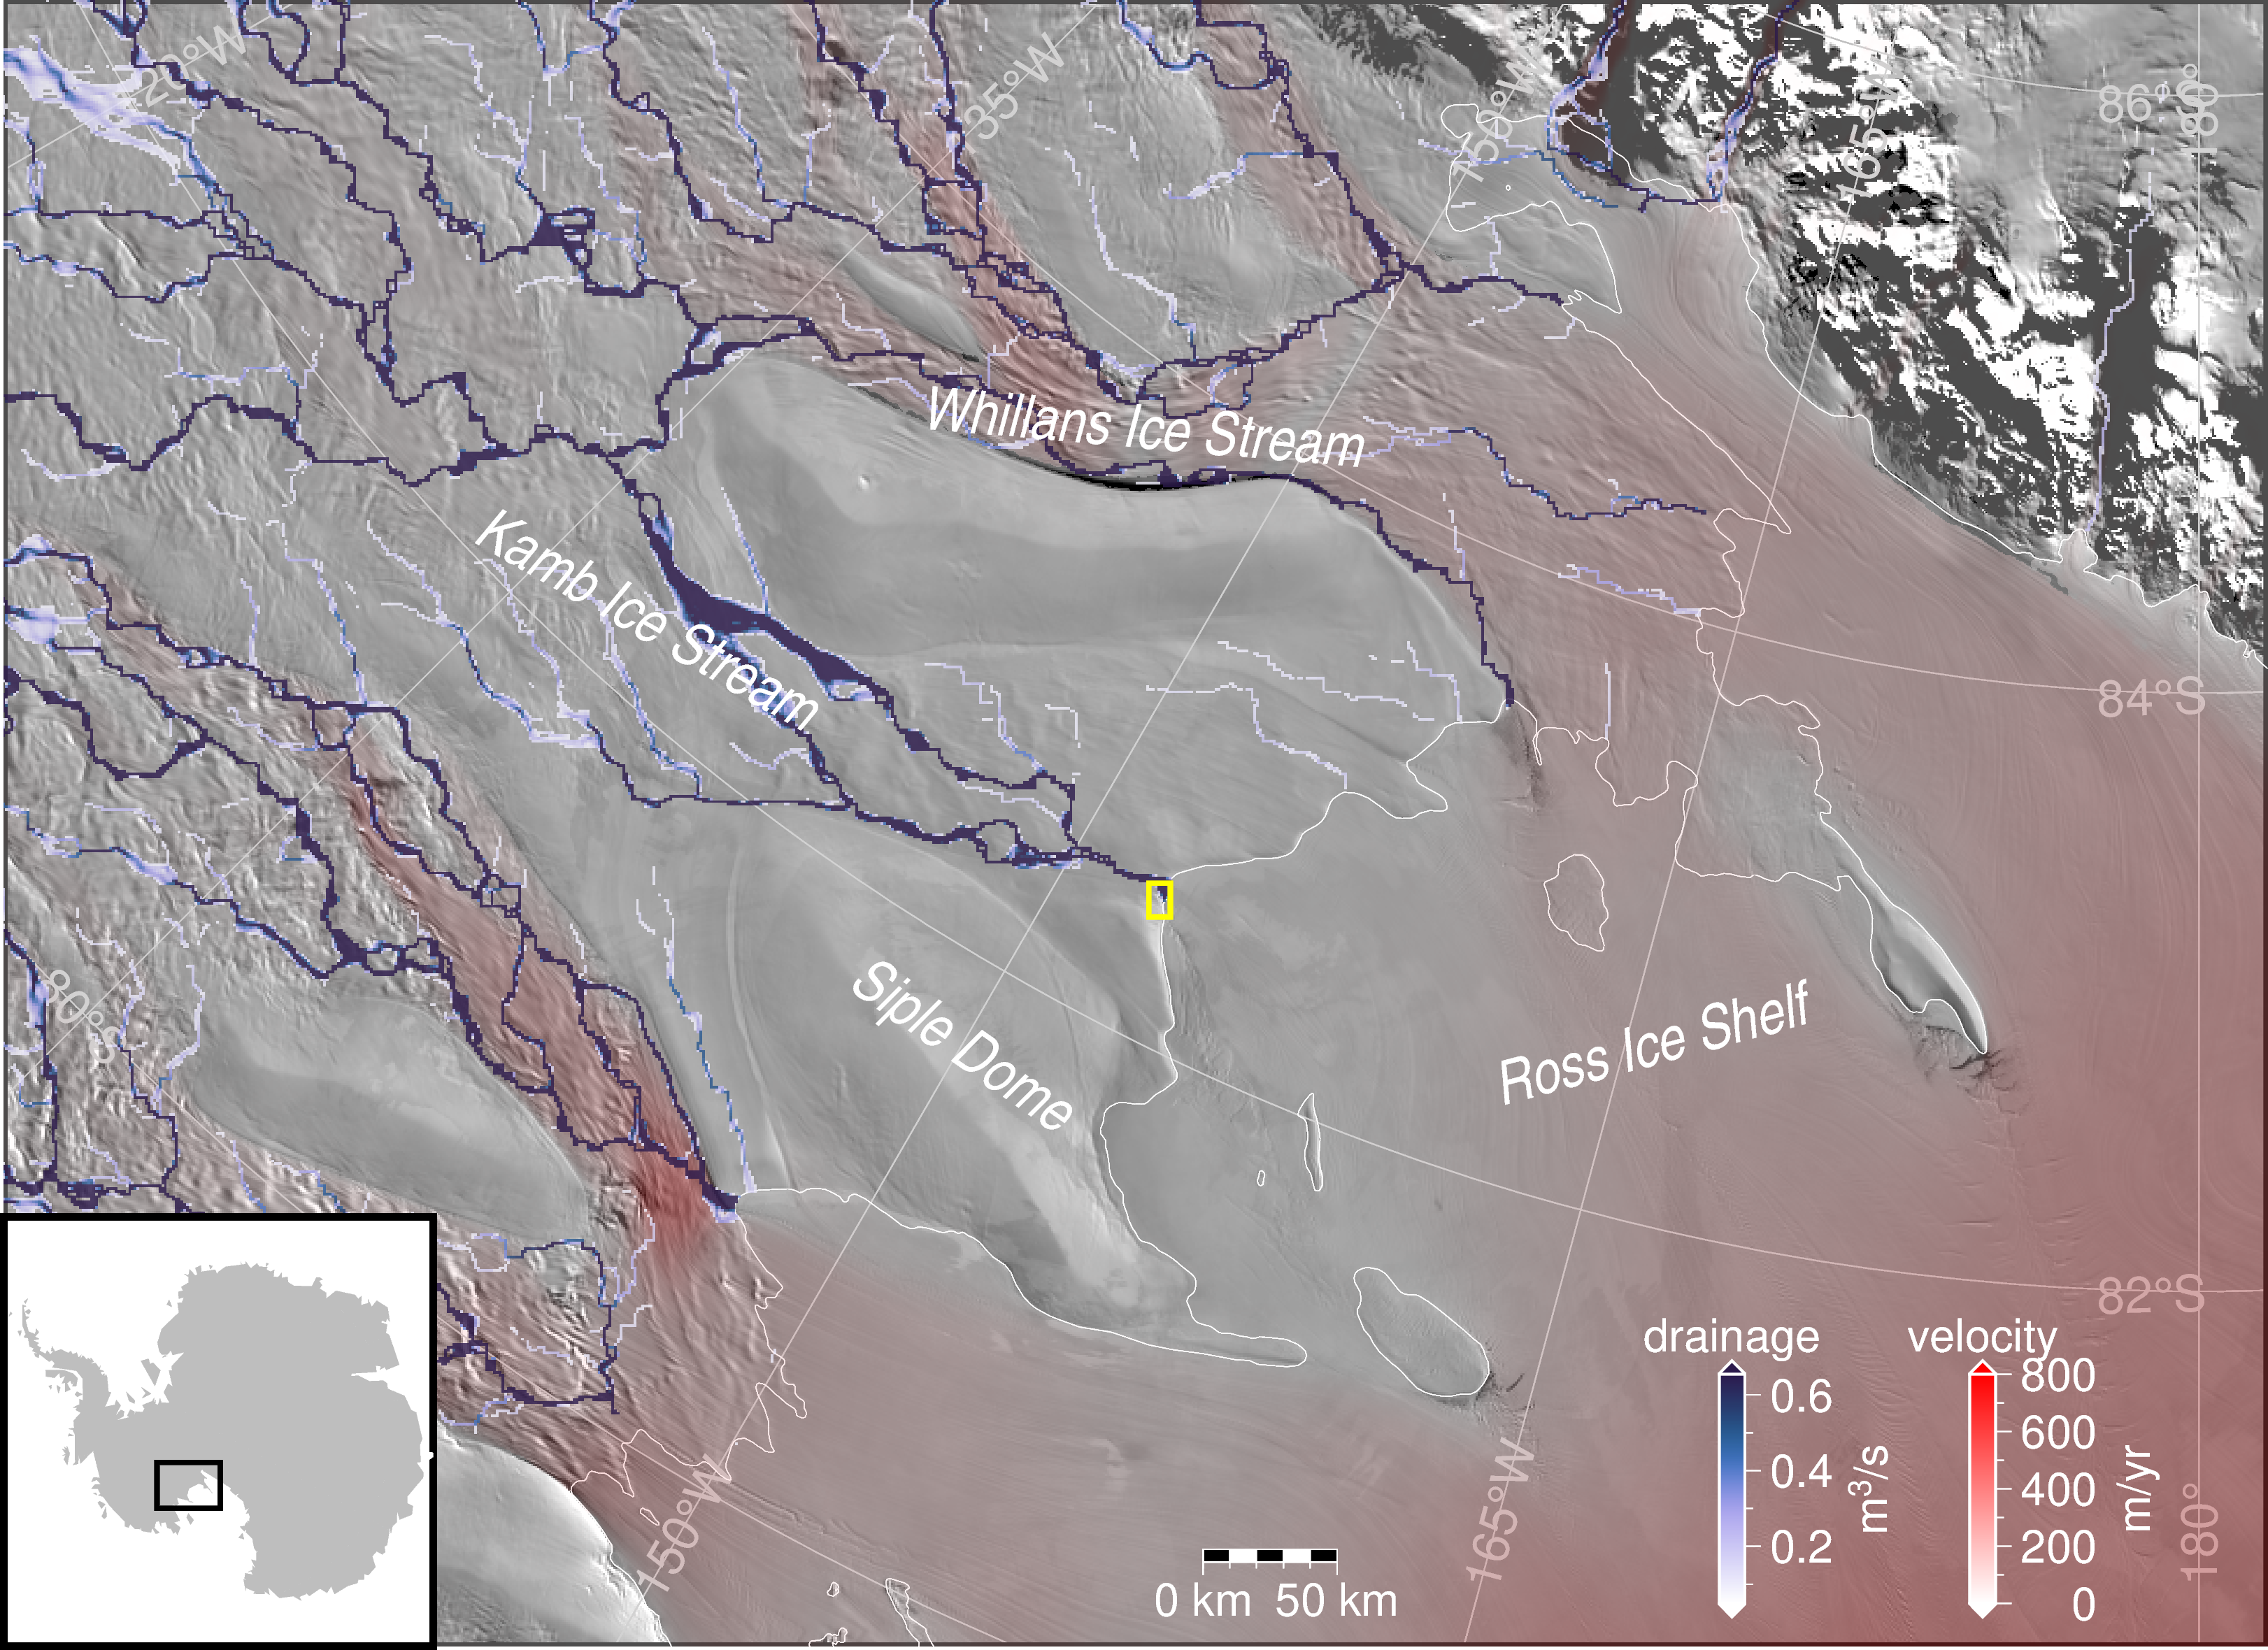
\includegraphics[width=1\textwidth]{chapters/2/fieldwork_location_small.png}
\caption[Fieldwork location]{Map showing the Siple Coast region. The study area is plotted as a yellow box at the grounding line of the Kamb Ice Stream. Figures \ref{fig:geophysics_overview}, \ref{fig:4square_channel}, and \ref{fig:thickness_surfacecolour} cover this study area. Modelled subglacial drainage of the Siple Coast is in blue \citep{le2009subglacial}, grounding line and coastline \citep{depoorter2013calving} are plotted as thin white lines. Background image is MODIS MOA 2009 \citep{haran2014modis} overlaid with MEaSUREs Phase-based Ice Velocity \citep{mouginot2019continent}. Antarctic place names are labelled in white. Figure produced using PyGMT \citep{uieda2021pygmt,wessel2019generic} with scientific colour maps \citep{crameri2018scientific}. Plotted using an Antarctic Stereographic Projection with a standard latitude of 71\textdegree S (EPSG:3031).}
\label{fig:fieldwork_location}
\end{figure} 

This study aims to further our understanding of subglacially--sourced channel formation. We present detailed observations of a basal channel at the grounding line of the Kamb Ice Stream (Figure~\ref{fig:fieldwork_location}).  Through these observations we aim to better constrain ice and ocean interaction in the channel, and processes which have formed the channel. These results be can used as a case study to further constrain models of channel formation and growth, and therefore their impact on ice shelves. The channel has been noted previously in literature \citep{alley2016impacts,kim2016active,goeller2015subglacial,horgan2017poststagnation}, and was profiled by airborne radar during Center for Remote Sensing of Ice Sheets (CReSIS) airborne radar project \citep{arnold2020cresis}. Because Kamb Ice Stream has little to no ice velocity, this channels is unique in that it is not formed by ice advection or shear. As a result, the channel can be used as a natural experiment in plume-driven melt processes. \cite{kim2016active} and \cite{alley2016impacts} suggested that the channel is formed from submarine melting from a subglacially sourced buoyant freshwater plume.  

We use the terms `surface valley' and `basal channel' to distinguish the surface and basal expressions of the channel respectively. `True left' and `true right' are from a perspective looking downstream. Channel `inception' refers to the upstream limit of the basal channel incision. Channel `apex' is the maximum height of along a lateral transect, while the `walls' are the channels lateral flanks. The `apex' and `walls' run down the length of the basal channel.  The surface valley lies at the downstream end of a modelled subglacial drainage path (Figure~\ref{fig:fieldwork_location}), and optical satellite imagery shows the feature is contiguous with a sinuous feature that cross--cuts streaklines upstream of the grounding zone (Figure~\ref{fig:moa_solo}). Downstream of the channel, the ice shelf exhibits a damaged zone many tens of kilometres long (Figures~\ref{fig:fieldwork_location},\ref{fig:moa_solo}).
In this paper, we start by examining the surface valley of the channel (Section~\ref{sec:surface}) using satellite imagery (MODIS MOA \cite{haran2014modis} and LandSat \cite{RoyLandsat8Scienceproduct2014}) and elevation products (REMA \cite{howat2019reference} and ICESat2 \cite{smith2021v3}), presenting surface elevation and surface elevation change. 
In Section \ref{sec:radar} we examine the basal channel underlying the surface valley, using low-frequency (7 MHz) radio--echo--sounding from a series of closely spaced (as little as 250 m) cross-channel profiles. Next, repeat phase sensitive radar (ApRES) observations are used to estimate the basal mass balance within the basal channel in Section \ref{sec:apres}.
We then discuss the implications of these results, first constraining the mechanism which creates the channel (Section \ref{sec:meltwater}), and explaining why we see discrepancies between the ice base and surface (Section \ref{sec:bridging}). We then estimate a lower bound on the melt rate magnitude in the basal channel (Section \ref{sec:melt}). 
Lastly, we discuss processes that could explain our observations. In particular, the linear shape of the channel (Section \ref{sec:retreat}), the steep shape of the channel inception (Section \ref{sec:steep}), and ledges in the channel (Section \ref{sec:side_melt}).



\begin{figure}[!ht]
\centering
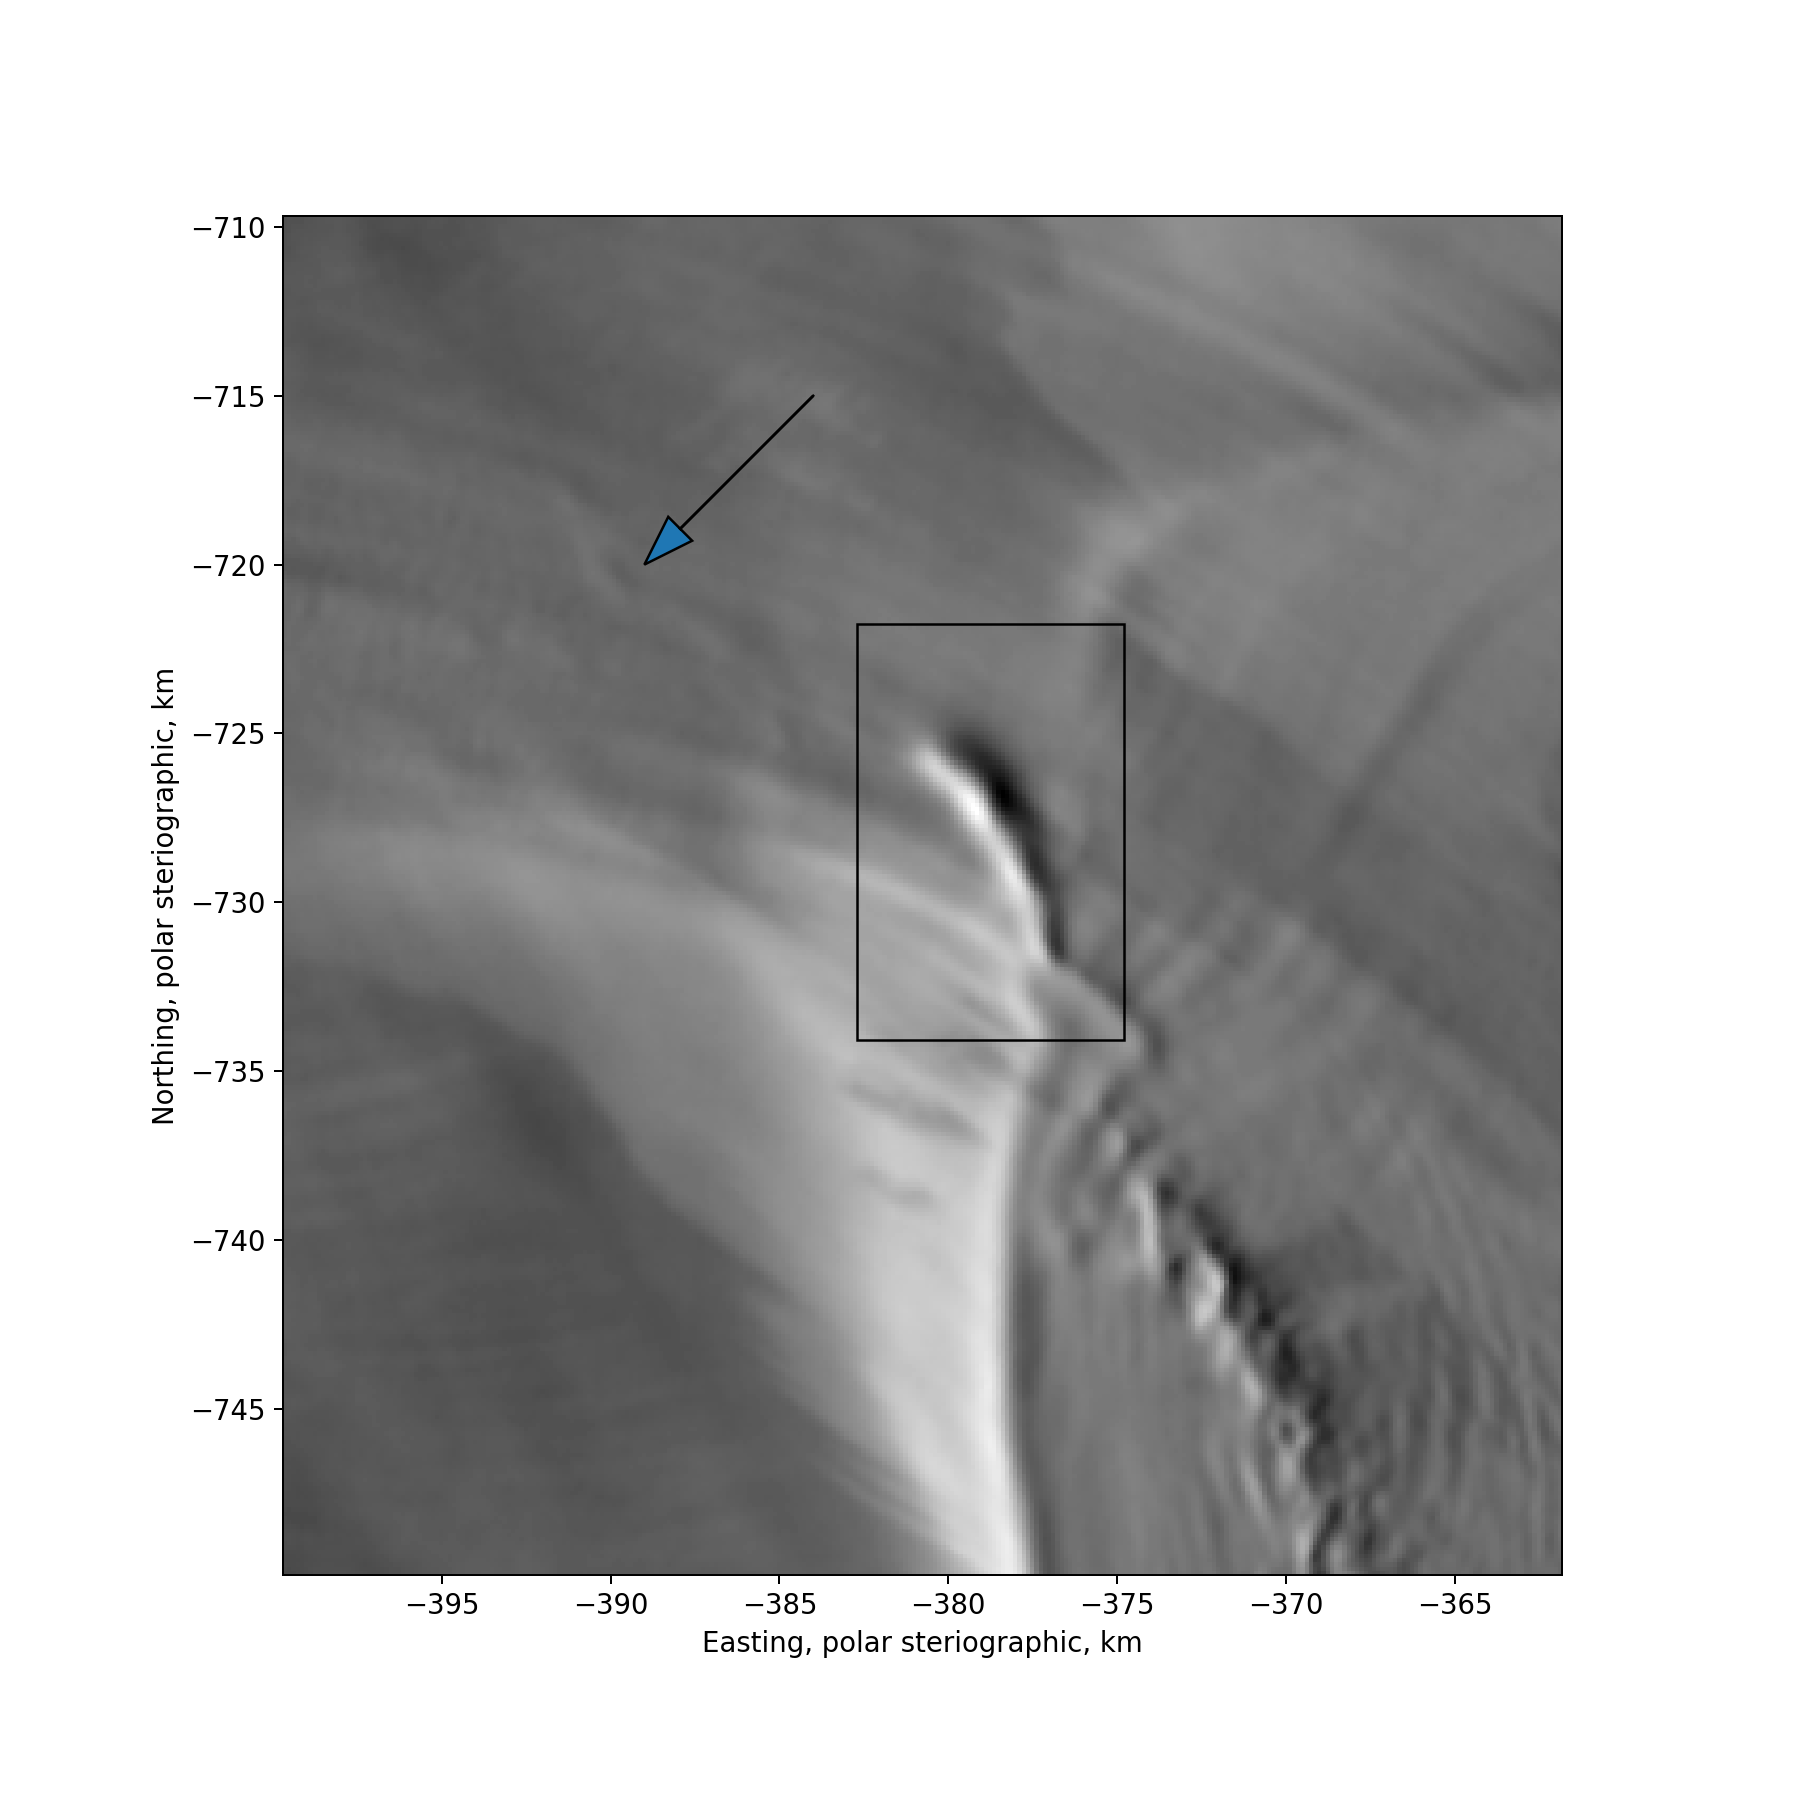
\includegraphics[width=1.0\textwidth]{chapters/2/moa_solo.png}
\caption[Image of valley]{MODIS MOA (2009) imagery of wider study area \citep{haran2014modis}. Arrow points to continuation of the surface valley upstream of the main study region. Black box outlines the study area shown in Figures \ref{fig:geophysics_overview}, \ref{fig:4square_channel}, and \ref{fig:thickness_surfacecolour}. }
\label{fig:moa_solo}
\end{figure}


\newpage

\section{Methods} \label{sec:method}

To estimate ice surface elevation and ice thickness in the study area we used a collection of remote sensing products and over-snow radio--echo--sounding. Basal mass balance is estimated at point locations using repeat ApRES. Data coverage is shown in Figure \ref{fig:geophysics_overview}. This section outlines the remote sensing products used and describes the ApRES and radio--echo--sounding processing along with the interpolation methods used to estimate ice thickness and ice base topography. 

%from DATA/Jupyter/PLOTS/ plots_kamb_data.ipynb
\begin{figure}[!ht]
\centering
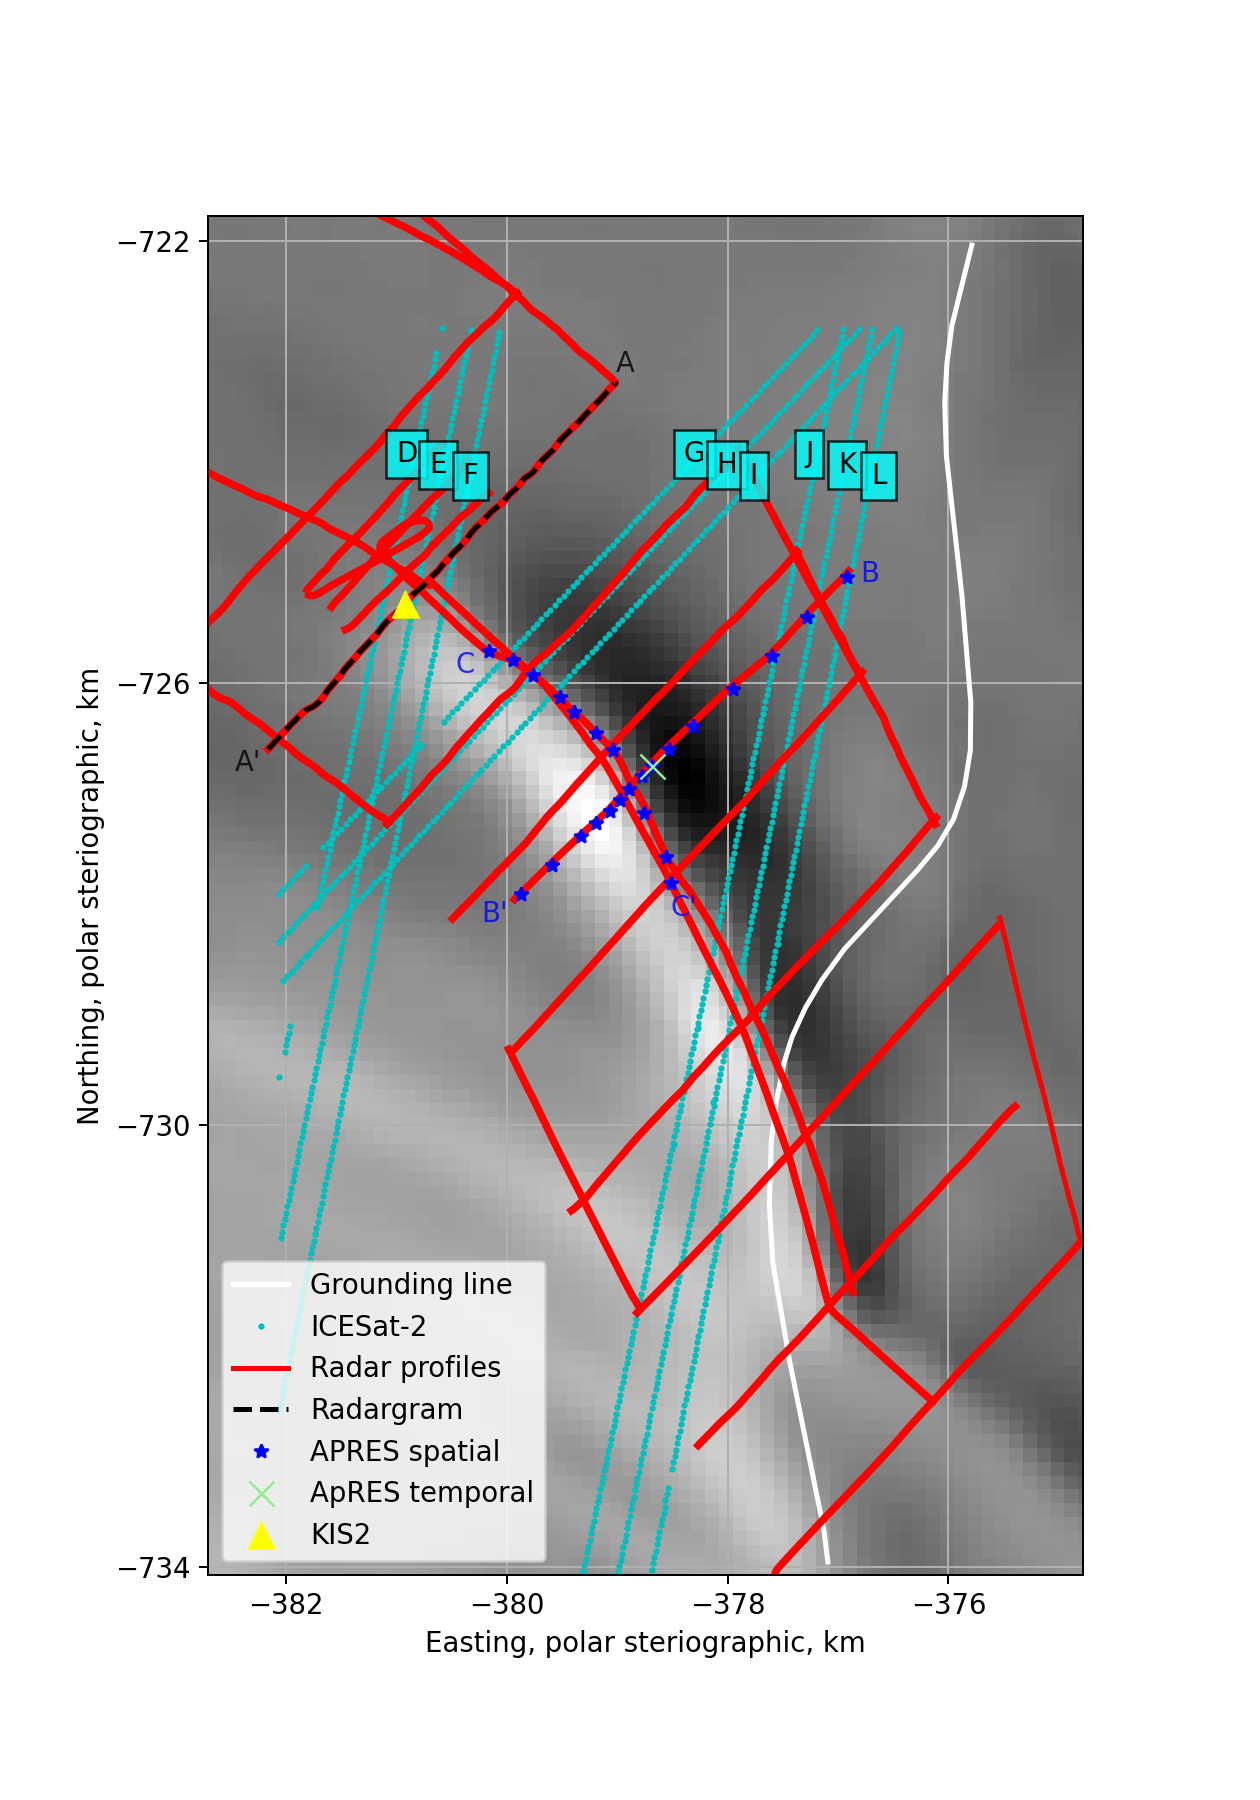
\includegraphics[width=0.8\textwidth]{chapters/2/geophysics_overview.png}
\caption[Map of field data]{Map of study area showing location of data. Ice flow direction is from top left to bottom right. Background image is MODIS MOA 2009 \citep{haran2014modis}. Red lines are low--frequency radar profiles, white line is grounding line from \cite{depoorter2013amii}, black dashed line shows location of radar profile from Figure S6, blue stars are ApRES repeat measurement locations, and light blue dots are ICESat--2 tracks.  ApRES was placed continuously recording at the light green `X', and the yellow triangle marks the planned location of a direct access drilling site scheduled for drilling in late 2021. Letters are referred to in subsequent figures.}
\label{fig:geophysics_overview}
\end{figure}


\subsection{Surface} \label{sec:surface}

\subsubsection{Remote Sensing} \label{sec:remote}

Four different remote sensing products were used to study the surface valley (Table \ref{tab:remote_table}). Optical satellite imagery included Landsat 4-8 \citep{RoyLandsat8Scienceproduct2014} and the 2009 MODIS Mosaic of Antarctica (MOA) \citep{haran2014modis}. Landsat 4, 5, 7, and 8 showed temporal change in the surface valley, and showed the earliest image of the valley in 1985. The 125 m spatial resolution MODIS MOA product provided a broader view of the study area and surrounding surface. For surface elevations, we used ICESat--2 and Reference Elevation Model of Antarctica (REMA) strips \citep{howat2019reference,smith2021v3}. ICESat--2 track coverage is shown in Figure \ref{fig:geophysics_overview}. REMA strips provided the most detailed view of surface elevation, with 2 m pixels over the study area. While nine strips from December 2012 to September 2017 pass over the study area, most have some cloud cover or miss a significant portion of the study area. The REMA strip from 9 November 2016 has full coverage, so was used used to calculate ice base elevation from ice thickness. A second REMA strip from 24 December 2012 was differenced from the 2016 strip to calculate the temporal gradient in the ice surface.
The 2012 and 2016 REMA strips state a vertical accuracy of 4 m and 3.5 m respectively \cite{noh2015automated,howat2019reference}. However, the elevation models are expected to be more accurate over the study area which is relatively stable due to low surface velocity \cite{rignot2017measures}.

We used ICESat--2 ATL11 point elevations \citep{smith2021v3}, which had nine tracks crossing the study area. The reference ground track numbers for these tracks are 114,  175,  349,  410,  617,  852, 1059, 1120, 1294. These were acquired more recently (since 2019) than the REMA elevation strips. Mean surface measurement precision from ATL11 points over the study area was 1.12 cm (Figure \ref{fig:icesat2_histogram}). For ICESat--2 differences a year apart, we double this mean surface precision to get an uncertainty of 0.02 m/yr.  All elevations in this paper are referenced to the GL04C geoid datum, which is approximately 47 m below the WGS84 ellipsoid datum in the study area.  Elevation differences from ICESat--2 ATL11 point elevations were also compared to differences calculated using debiased REMA strips.

\begin{figure}[!ht]
\centering
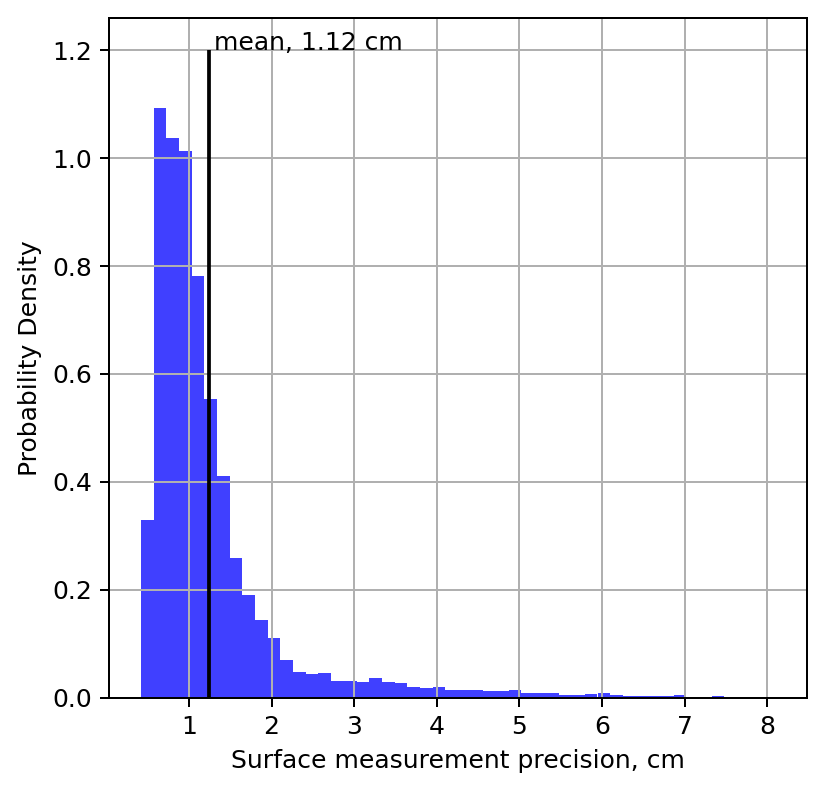
\includegraphics[width=0.9\textwidth]{chapters/2/icesat2_histogram.png}
\caption[ICESAT--2 surface measurement precision]{Histogram showing the range of ICESAT--2 surface measurement precision in the study area.}
\label{fig:icesat2_histogram}
\end{figure}



% In REMA difference data, this observed raising is the same sign as the general trends and error over the REMA strip (Figure S11, S12). This increases the likelyhood that the observations are artefacts. However, the close coincidence of similar raising in the more accurate ICESat--2 data supports the observation.
% 



%%%%%%%%%%%%%%%%%%

\begin{table}
\centering
\begin{tabular}{ |c|c c c| } 
 \hline
 Product & Data timespan & Site coverage &  Reference \\ 
 \hline
%  \hline
 REMA 2m strip &  12/2012--09/2017 & 2 m pixels of site area 
 & \cite{howat2019reference}\\ 
%  \hline
 ICESat--2 &  4/2019--ongoing &  6 tracks across channel  & \cite{smith2021v3}\\
%  \hline
 Landsat &  1985--ongoing & 20 m pixels covering site area  & \cite{RoyLandsat8Scienceproduct2014}\\ 
%  \hline
 MODIS MOA & - & 125 m pixels covering site area  & \cite{haran2014modis}\\
 \hline
\end{tabular}
\label{tab:remote_table}
\caption{Remote sensing products used in this study.}
\end{table}


\subsection{Ice thickness} \label{sec:icethickness}

\subsubsection{Low Frequency Radar} \label{sec:radar}


\begin{figure}[!ht]
\centering
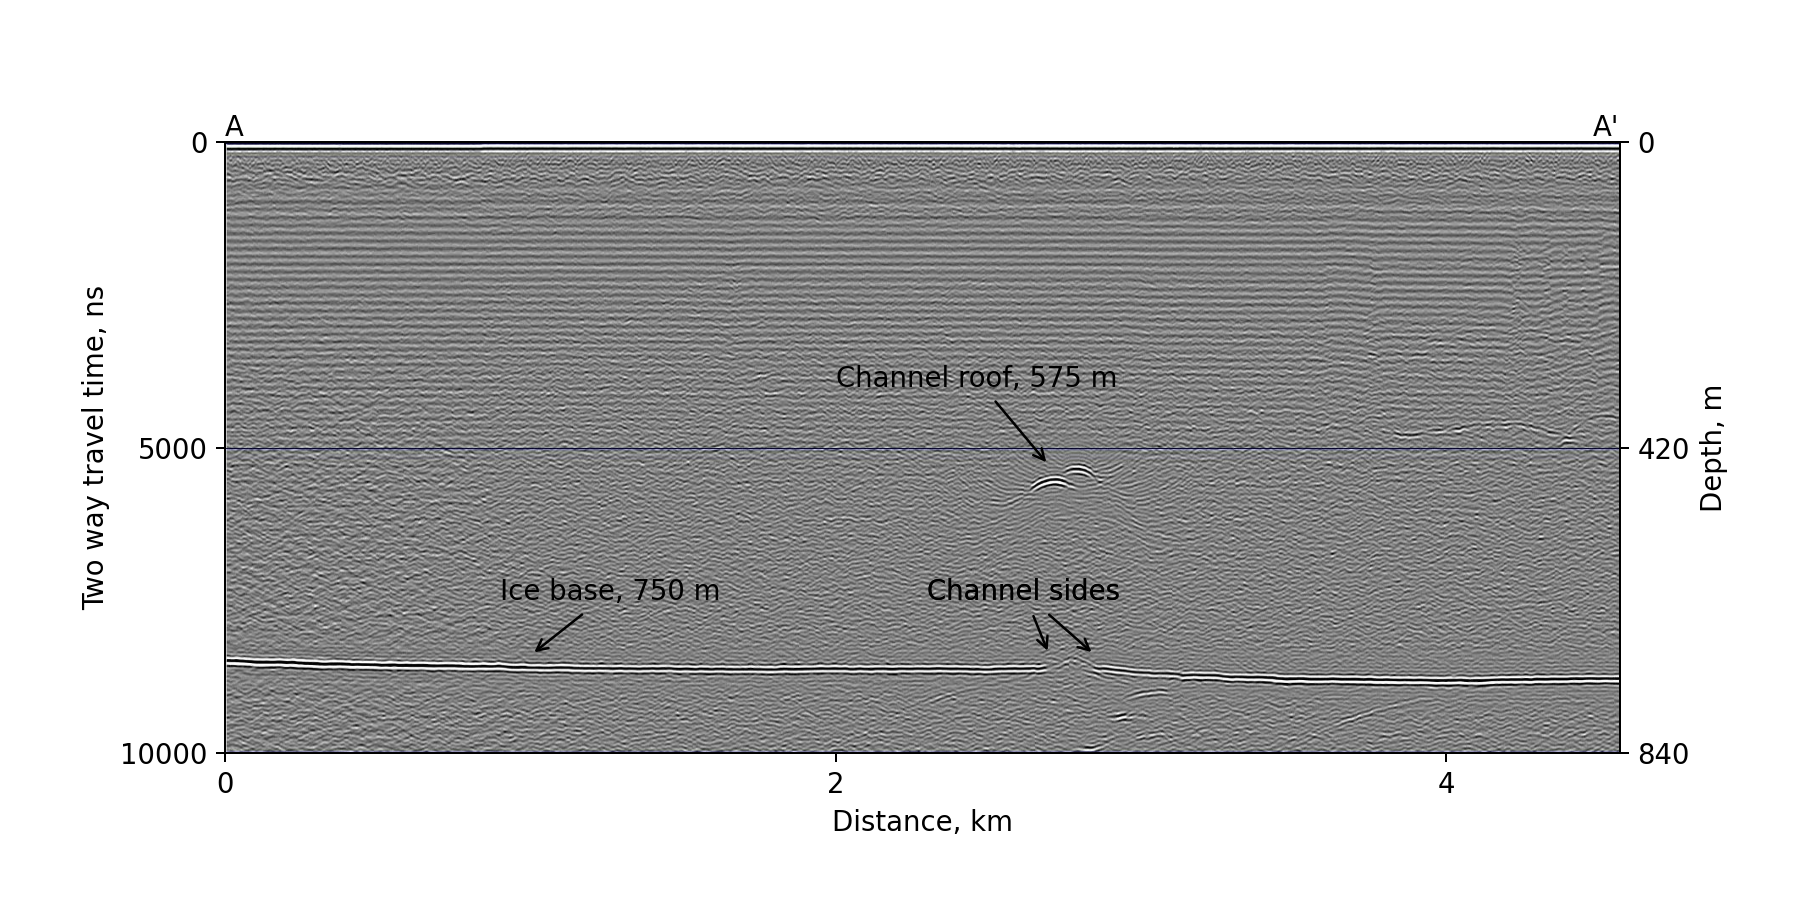
\includegraphics[width=1.1\textwidth]{chapters/2/radargram.png}
\caption[Example radargram]{Processed radargram showing radar reflection of the basal channel. Profile location is shown as a black dashed line in Figure \ref{fig:geophysics_overview}.}
\label{fig:radargram}
\end{figure}

To estimate ice thicknesses over the channel, the study area was profiled using low-frequency (7 MHz) radio--echo--sounding.  Radar profiles were 1000-1400 m apart, except at the head of the channel where the spacing between lines was reduced to approximately 200 m to better constrain the inception of the channel (Figure~\ref{fig:geophysics_overview}). %In the 2019--20 Antarctic field season  This followed a preliminary radar survey of the channel four years prior. 
Data collection followed \cite{christianson2016basal}. The radar transmitter and receiver were towed on sleds at approximately 8 km/hr resulting in an average spatial resolution along radar lines of 1.8 m. Data processing included dewowing, bandpass filter (1-2--15-18) MHz, along track spatial stacking into 3 m bins, and debiasing. The data were then finite difference migrated at 169 m/$\mu$s, before a final (3-4-15-18) MHz bandpass filter was applied. The resulting profile data in off-nadir reflections (discussed in more detail in \cite{christianson2016basal}), which are difficult to interpret but must be considered during analysis.  Radar survey positioning used Global Navigation Satellite Signal (GNSS) observations, post processed using the Precise Point Positioning kinematic method \citep{ppp2016}. An example processed radar line is shown in Figure \ref{fig:radargram}. The location of all radar lines are shown in Figure \ref{fig:geophysics_overview}.
Following \cite{dowdeswell2004investigations}, a firn correction of +7 m was added to ice thickness. Additionally, a +7 m was added to ice thickness to correct the offset between the single frequency radar and the more accurate ApRES ice thicknesses. This difference is likely caused by the low frequency radar trigger threshold. This correction was calculated as the mean difference between ice thicknesses derived from coincident ApRES and low frequency radar at line BB' shown on Figure \ref{fig:geophysics_overview}.

\subsubsection{Ice base DEM} \label{sec:interp}

We estimated the three dimensional shape of the basal channel by digitising the base of the ice and then interpolating between radar profiles. Our observations of ice thickness had high spatial sampling across the channel (3 m trace spacing) and low spatial sampling in the downstream direction (profile spacing of 200--1400 m). This meant that conventional interpolation techniques failed to capture the shape of the steep sided narrow channel (Figure \ref{fig:gmt_surface_interp}). To overcome this we use an interpolation method that is based on the assumptions that the channel is bounded laterally and has downstream continuity. First, all radar lines crossing  the channel were resampled spatially from the channel apex to either side of the channel. Equivalent points from each line were then interpolated downstream with a cubic spline. These along--channel interpolated  profiles were then interpolated altogether onto a regular grid.  Because radar lines parallel to the channel included some off-nadir reflections that were not correctly repositioned by migration, they were not used in the interpolation. Ice thickness in the study area not over the channel was estimated using linear interpolation of all radar line points outside the channel. The channel thickness interpolation was cropped onto the surrounding ice thickness estimate, and the whole study area was again gridded using a nearest--neighbour interpolation. The resulting estimate of ice thickness (Figure \ref{fig:thickness_solo}) was then subtracted from a 2 m REMA surface elevation strip to produce ice-base elevation.
Our interpolation technique accounts for the anisotropic resolution of radar data by assuming that the cross section of the channel has downstream continuity. Additionally, it uses the cross-channel radar profiles which unlike downstream profiles can be corrected by 2D migration, and so give a more accurate quantification of ice base elevation. 
The resulting interpolation of the basal channel shape was compared to  independent basal elevation estimations provided by Center for Remote Sensing of Ice Sheets (CReSIS) airborne radar project \citep{arnold2020cresis}, which had three lines passing over the basal channel in the study area.  

One goal of estimating an accurate channel shape is to better constrain the freshwater plume which carves the channel. For this, the gradient of the channel inception is important, as it is a dominant forcing in plume melt rate models \citep{jenkins1991one}. Locating the inception of the channel, however, is not straightforward due to off nadir reflections. The channel inception is best shown in a radar line parallel to channel direction (Figure A \ref{fig:radarlines_surfcoloure}). From this, we deduce that the farthest upstream radar line which has a reflection crossing the channel, shows an off nadir reflection. This interpretation is confirmed by the fact that this radar data shows a reflection distance equal to the distance to the channel reflection on the next radar line.  In the channel interpolation, the channel depth is set to be zero at this off nadir reflection, which constrains the downstream distance or angle over which the channel forms.



\subsubsection{Hydrostatic Equilibrium} \label{sec:float}

For each pixel from the ice base DEM, we calculated the vertical distance which the ice column is offset from hydrostatic equilibrium. We call this the vertical offset from hydrostatic equilibrium.
An offset of zero describes ice at hydrostatic equilibrium (described in Section \ref{sec:float}), and a negative/positive offset indicate the ice column is held below/above equilibrium by external forces.
To calculate this measure we first estimated average density of the ice column for each pixel, using ice thickness from the interpolated DEM (Section \ref{sec:interp}) and the density-depth model of \cite{herron1980firn}. For the density model, we assumed an accumulation rate of 0.11 m/yr \citep{craig_personal_comm}, a mean annual temperature of -27.3 \textdegree C, and initial, critial and ice densities of 300, 555 and 917 kg/$\mathrm{m}^2$ respectively.
Next, using Archemedis principle, ice thickness and average density, we calculated the theoretical freeboard if the ice column at each pixel were at hydrostatic equilibrium. This is calculated as $h_{freeboard} = h_{thickness} \left( 1 - \bar{\rho_i}/\rho_s \right)$ where $h_{freeboard}$ is the freeboard elevation of the pixel at hydrostatic equilibrium, $\bar{\rho_i}$ is the average density of the ice column for a pixel and $\rho_s$ is the density of displaced seawater which we set to 1030 kg/$\mathrm{m}^2$. We subtracted the resulting freeboard elevation from the the REMA elevation of the region corrected to the GL04 geoid to get the vertical offset from floatation (Figure \ref{fig:bridging}).  

\subsubsection{ApRES} \label{sec:apres}

Basal mass balance was surveyed using ApRES on two profiles, one parallel to the surface valley low, the other crossing the channel (Figure \ref{fig:geophysics_overview}). ApRES observations were made in Dec 2019 and repeated in Dec 2020 at the same locations, which we marked with flags. The ApRES antennae had a parallel orientation and were spaced 9 m apart. Data collection and processing followed the method described in \cite{stewart2019basal}. The ApRES surveys are not migrated so results may show off nadir reflections.
While the ApRES can observe accretion, quantifying the rate is problematic due to the occurrence of multiple reflections from both the glacial/marine--ice interface and the marine--ice/water interface, and unknown changes in the properties of marine--ice  \citep{vavnkova2021nature}. The values presented should be interpreted as an `apparent accretion' rate as described by \cite{vavnkova2021nature}.

%If these reflections are close together they cannot be distinguished and the coherent sum of these reflections gives a phase shift depending on the thickness of the layer, its permittivity, and the relative strength of the internal and basal reflections.  
%By assuming that the nature of the accretion, the salinity and ice volume fraction, is similar between sites we can compare the relative size of accretion. 

\newpage

\section{Results} \label{sec:results}

\subsection{Topography} \label{sec:topography}

\subsubsection{Surface topography} \label{sec:surfacetopog}
%The basal channel is manifest on the surface of the ice as a valley. 
The surface valley is visible in the first available imagery from Landsat 5 in 1985 and extends further upstream in subsequent Landsat imagery in 1989, 2002, and 2020 (Figure \ref{fig:historic}). While changing illumination angles may affect the apparent migration of the valley, the apparent migration appears to exceed any direct shading effects. By 2020 the channel appears more defined and extends approximately 1.5 km upstream of the 1985 surface channel. The 2016 REMA strip shows that the surface valley was approximately 2 km wide, over 10 km long and had a maximum depth of 15 m relative to the adjacent ice stream (Figure \ref{fig:4square_channel} B).  The valley starts abruptly, 5 km inland from the \cite{depoorter2013amii} grounding line (Figure \ref{fig:geophysics_overview}). The surface gradient at the head of the valley is approximately -1 degree, then the valley is fairly straight and flat--bottomed for around 1.5 km. The valley then becomes moniliform, with three connected distinct basins downstream (labelled B1, B2, B3 in Figure \ref{fig:thickness_surfacecolour}).
The three basins downstream from the surface valley inception correspond to bends in the basal channel. Both the surface valley and basal channel first turn to the true right by 30 degrees (B1), then right by 20 degrees (B2) then left by 60 degrees (B3) at the three basins respectively. On the surface, high points between basins are 3-7 m higher than the basin lows, and the valley is 5-10\% wider at the basins.
In historic imagery (1985, 1989; see Figure \ref{fig:historic}) the three basins are visible, and the surface valley does not extend upstream from the three basins. 

In the 2009 MODIS MOA imagery, a faint trace of the valley continues upstream from its clear head for 10 more kilometres (Figure \ref{fig:moa_solo}). The faint trace of the basal channel upstream is not visible in radar profiles. 

\begin{figure}[!ht]
\centering
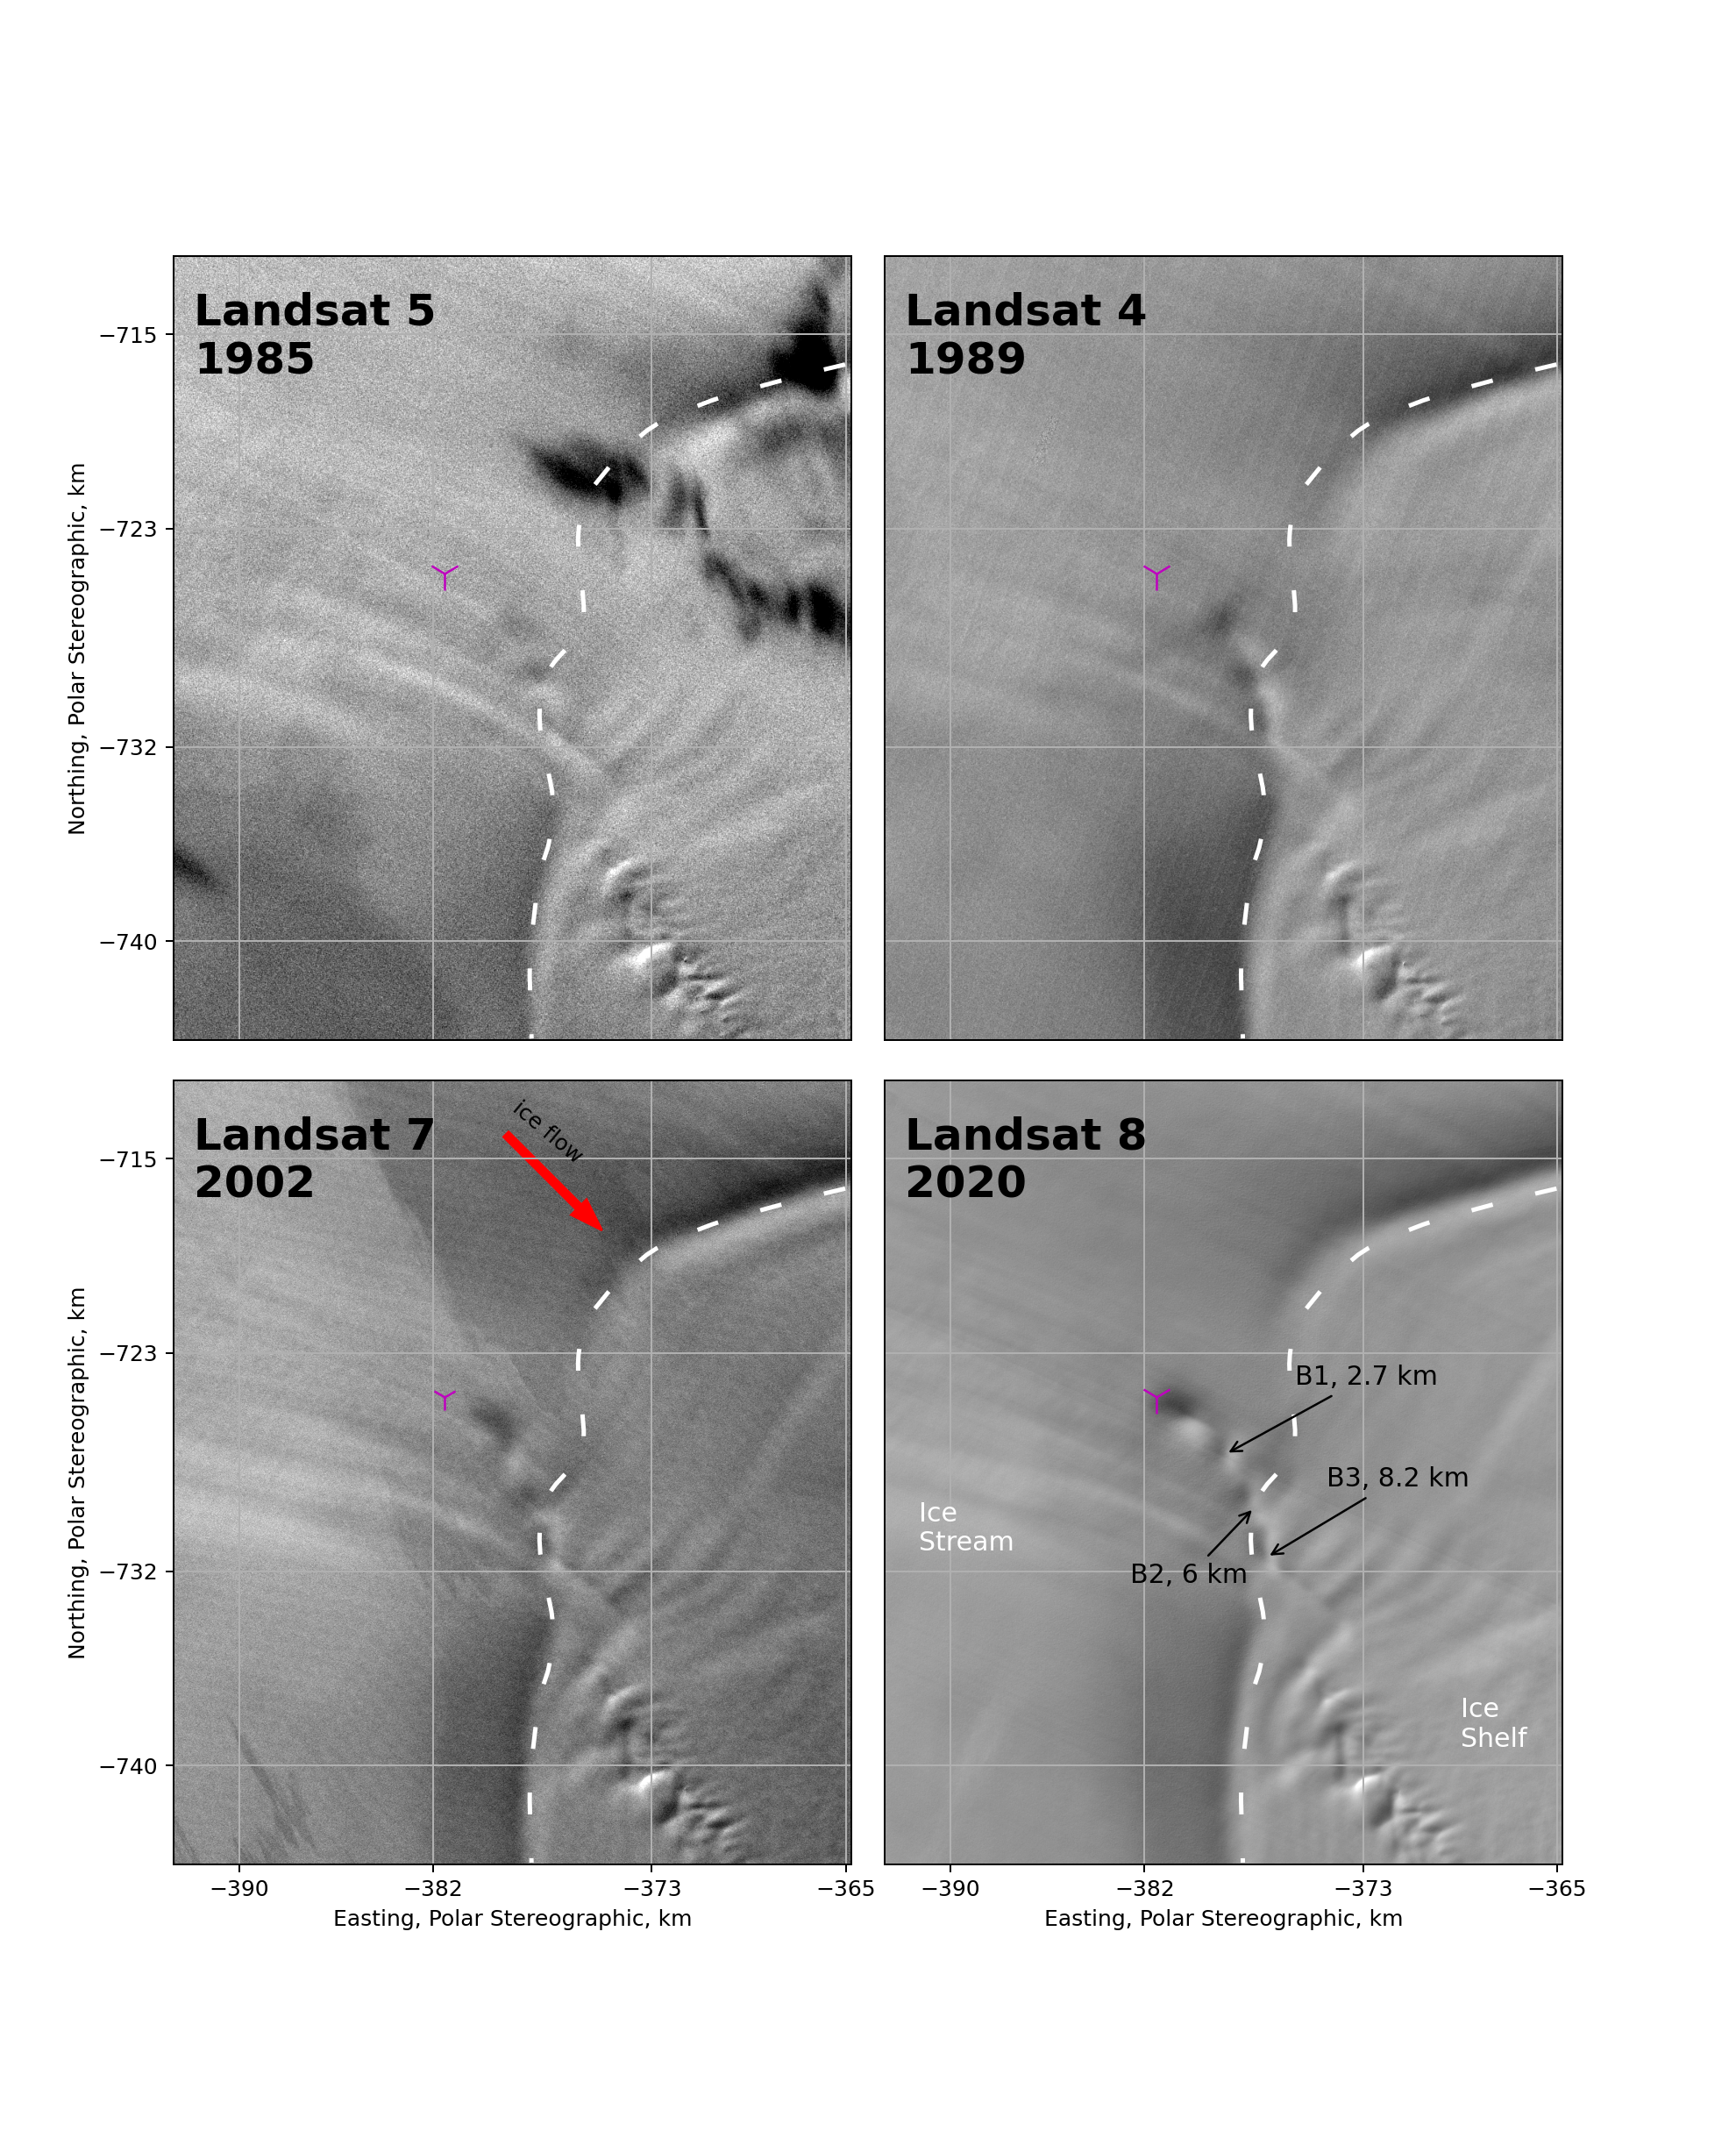
\includegraphics[width=1\textwidth]{chapters/2/historic_channel.png}
\caption[Historic Landsat imagery]{Landsat imagery of a visible valley in the ice surface \citep{RoyLandsat8Scienceproduct2014}, shown in the central grid square at (-380,-725 km). The surface valley sits at the outlet of estimated subglacial drainage paths (Figure \ref{fig:fieldwork_location}), and is the surface expression of a sub--ice--shelf channel. The grounding line \citep{depoorter2013calving} is shown as a white dashed line, which divides the Kamb Ice Stream and the Ross Ice Shelf. Red arrow shows direction of ice flow. Basins B1--3 are topographic lows in the ice surface, distances are  from the upstream start of the Interpolated Channel Maximum to each basin centre.}
\label{fig:historic}
\end{figure}




%/DATA/Jupyter/PLOTS/data_paper/05_4square_channel.ipynb
\begin{figure}[!ht]
\centering
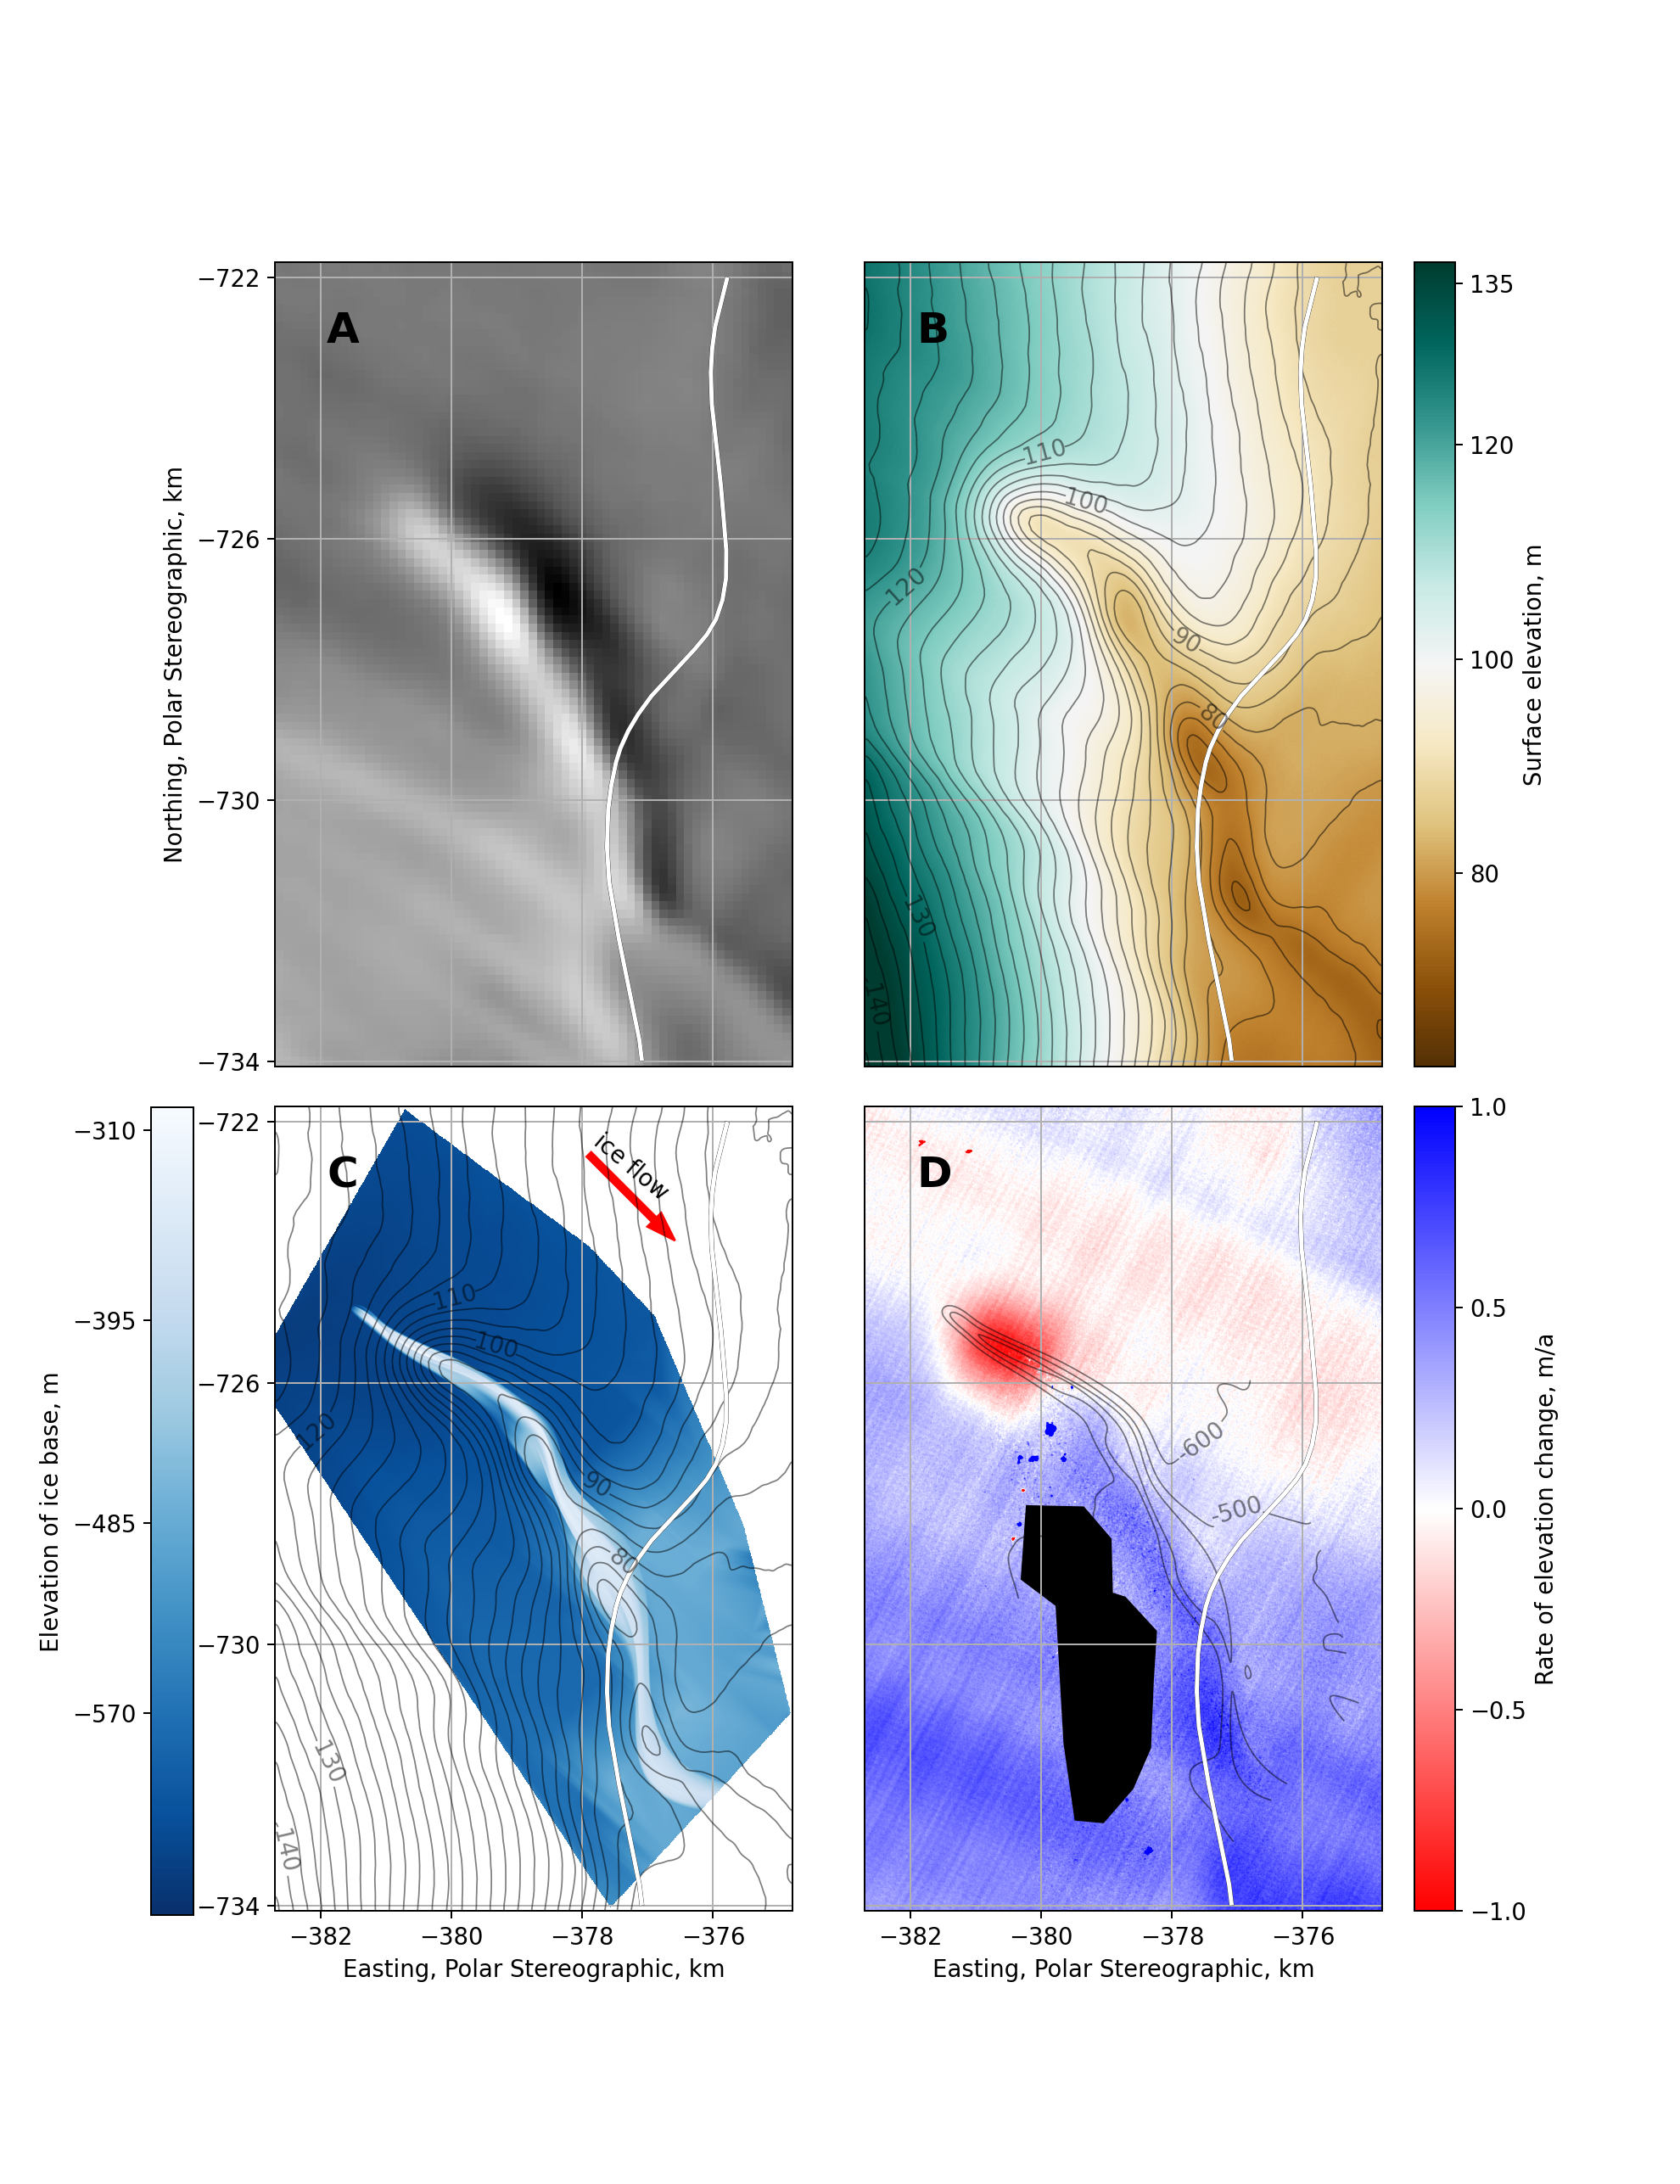
\includegraphics[width=0.9\textwidth]{chapters/2/4square_channel.png}
\caption[Channel observations]{A: MODIS MOA optical image of study area \citep{haran2014modis}. B: REMA ice elevation, 2 m resolution, \citep{howat2019reference}. The white line is the grounding line from \cite{depoorter2013amii} C: Estimated ice base elevation interpolated from radar survey, contours of REMA surface elevation.  D: Difference between REMA elevation from 2012-12-24 to 2016-11-09, contours show estimated ice base.  Red line shows direction of ice flow. Black area is masked out due to clouds.}
\label{fig:4square_channel}
\end{figure}  

\subsubsection{Ice base topography} \label{sec:icebasetopog}

\begin{figure}[!ht]
\centering
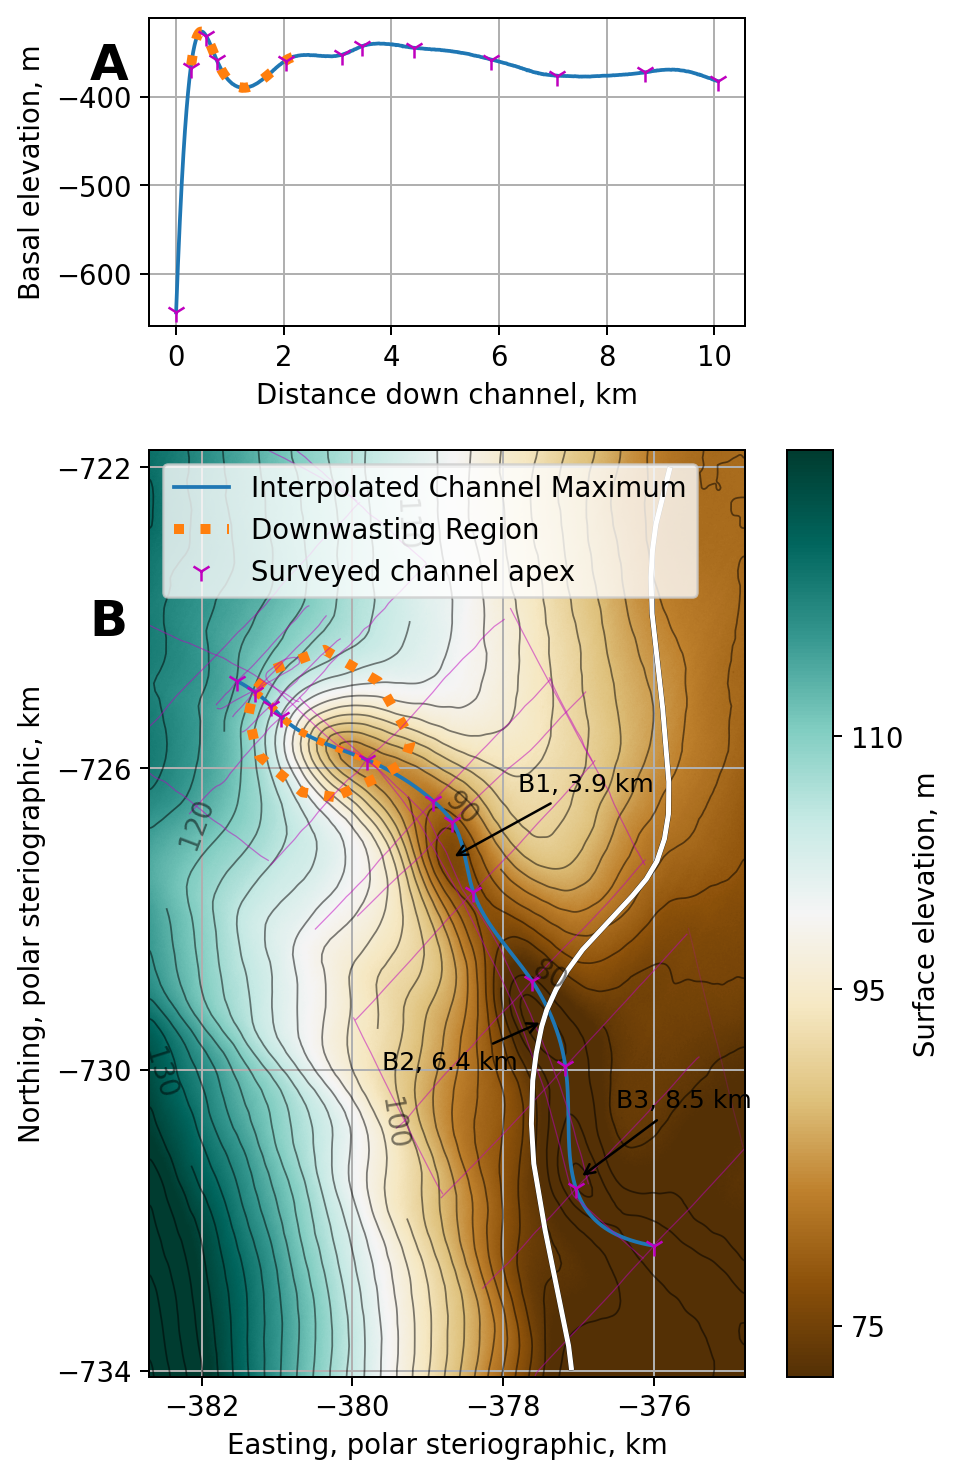
\includegraphics[width=0.8\textwidth]{chapters/2/thickness_surfacecolour.png}
\caption[Ice base profile]{A) Estimated ice base elevation along the apex of the channel, calculated by interpolating between the maximum height of each radar line crossing the channel (Surveyed channel apex). B) Estimated channel apex position plotted over REMA surface elevation. Basins B1--3 are topographic lows in the ice surface, distances are from the upstream start of the Interpolated Channel Maximum to each basin centre. The region of surface lowering is delineated by orange dotted region, and coincides with the onset of the surface valley. White line is the grounding line from \cite{depoorter2013amii}.}
\label{fig:thickness_surfacecolour}
\end{figure}  

The downstream profile of the channel apex is best described from radar lines perpendicular to the channel. Radar lines following the channel do not accurately show channel depth due to off nadir reflections.  The bisection of perpendicular radar lines and the channel apex are shown in Figure \ref{fig:thickness_surfacecolour} as `Surveyed channel apex' and are interpolated to produce the `Interpolated Channel Maximum' as described in Section \ref{sec:interp}.  The `Surveyed channel apex' show the basal channel starts abruptly, approximately 300 m upstream from the start of the surface valley (Figure \ref{fig:thickness_surfacecolour} B). The inception of the basal channel inclines from 0 m to 300 m above the bed over less than 300 m horizontally, constrained by the spacing between parallel radar profiles. Therefore, the initial gradient of the basal channel is constrained as between 45 and 90 degrees from horizontal. Over 500 m downstream the basal channel incises approximately 50\% of ice thickness (350 m of 700 m), to a maximum elevation of -325 m (Figure \ref{fig:thickness_surfacecolour} A).
The `Surveyed channel apex' then show a reduction in basal channel height of greater than 30 m to an elevation of -330 m at 0.75 km downstream from its inception (Figure \ref{fig:thickness_surfacecolour} A). The interpolated channel maximum estimates a local minimum in the downstream channel apex at -390 m elevation, 1.25 km downstream, though this is unsupported by data points.  The `Surveyed channel apex' show that the basal channel apex rises to around -340 m at 3.5 km then lowers to around -380 m at 10 km (Figure \ref{fig:thickness_surfacecolour} A) at the edge of the study area. The elevation of the surface valley is at approximately 80 m (Figure \ref{fig:thickness_surfacecolour} B). 
%continues at 430m below 

The basal channel has three bends which correspond to surface basins B1--3 (described in Section \ref{sec:surfacetopog}). The channel is around 200 m wide for almost 1 km from its inception, then widens to 700 m at the first bend (B1) 3.9 km down the channel, narrows to 450 m then widens to 1050 m at the bend (B2) 6.4 km downstream (Figure \ref{fig:4square_channel}). These widths are measured at radar lines and are therefore not a result of interpolation. While there are no radar lines crossing the channel at the third bend (Figure \ref{fig:ice_base_solo}), the interpolation estimates that the basal channel narrows to 200 m and widens to 600 m at the third bend (B3) 8.5 km downstream (Figure \ref{fig:4square_channel}). While these bends correspond to basins in the surface elevation, they do not correspond discernibly to changes in the ice base elevation. 
\begin{figure}[!ht]
\centering
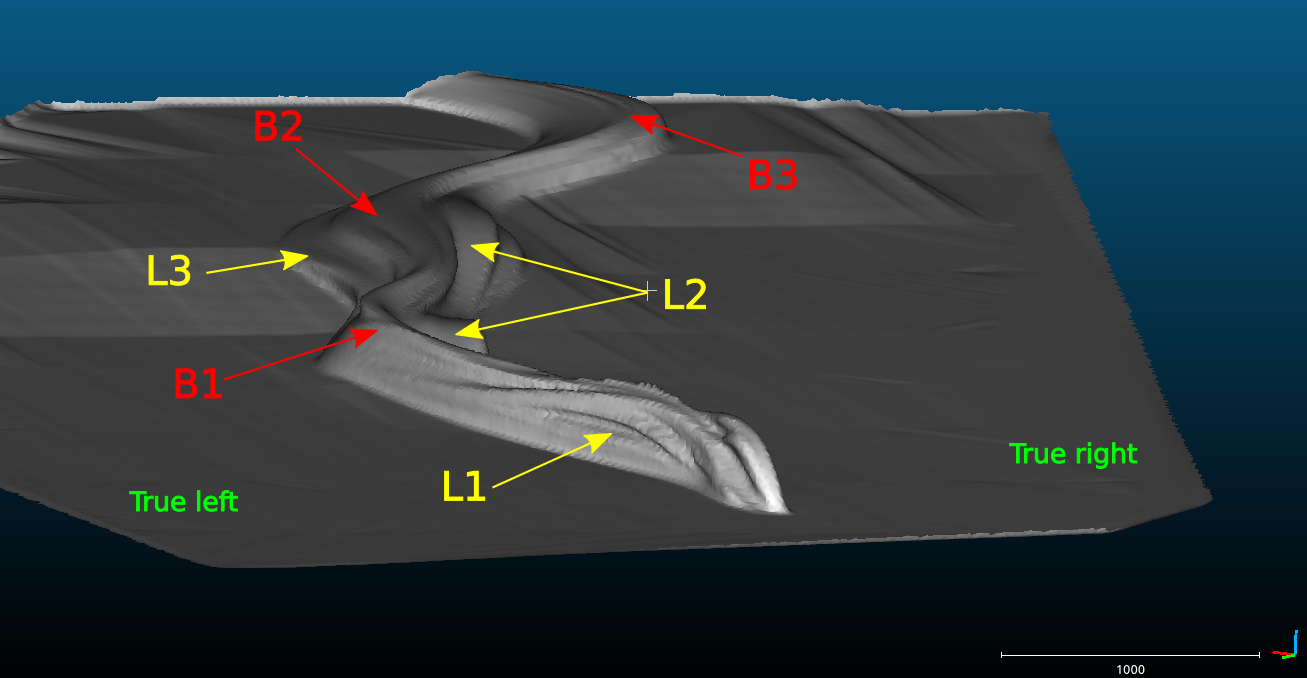
\includegraphics[width=1.1\textwidth]{chapters/2/ledges1.png}
\caption[3D ledge view (A)]{Three dimensional view of the ice base map, showing the location of ledges (L1, L2, L3) and bends in the channel (B1, B2, B3). Bends correspond to basins on the subaerial ice surface.}
\label{fig:ledges1}
\end{figure}

\begin{figure}[!ht]
\centering
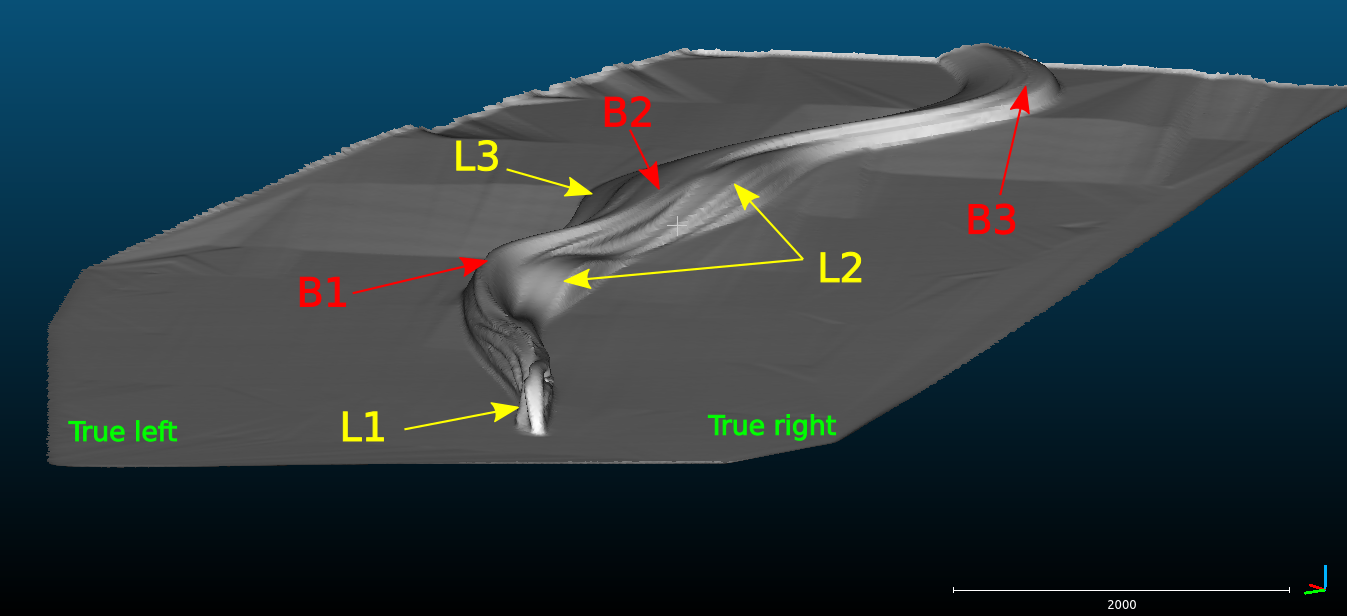
\includegraphics[width=1.1\textwidth]{chapters/2/ledges2.png}
\caption[3D ledge view (B)]{Three dimensional view of the ice base map, showing the location of ledges (L1, L2, L3) and bends in the channel (B1, B2, B3). Bends correspond to basins on the subaerial ice surface.}
\label{fig:ledges2}
\end{figure}

The cross--sectional shape of the basal channel varies along flow. While the basal channel flanks are imaged to be consistently vertical, the channel has distinct ledges along its sides (Figure \ref{fig:ledges1}). These ledges are separated from the apex of the basal channel by a vertical offset. For around 1 km downstream of the basal channel inception, a ledge is visible on the true left (Figure \ref{fig:ledges2}, L1), this is separated from the basal channel apex by a wall ranging from 200 m at first to 50 m further downstream. A ledge on the true right then appears from around 1 km to 6 km downstream from the channel inception (Figure \ref{fig:ledges1}, L2). This ledge is widest at the bend (B1) 3.9 km downstream from the channel inception  where it is 150 m shallower than the channel apex. A third ledge (Figure \ref{fig:ledges1}, L3) is visible from 4 to 6.6 km downstream  from the channel inception.  The last 4 km of the channel has no observable flat ledges and the channel walls appear to have a gentler slope than those upstream.

\subsubsection{Hydrostatic Equilibrium} \label{sec:floating}

The basal channel inception appears approximately 6 km upstream of the grounding line estimated by \cite{depoorter2013amii}. 
The vertical offset of the ice column from hydrostatic equilibrium indicates where the ice is freely floating and ranges from -10 to 45 m over the study area (Figure \ref{fig:bridging}).
A positive vertical offset denotes an ice column which is held above floatation, either by the ground or from internal ice stresses. A vertical offset of zero denotes ice which is floating, and a negative vertical offset denotes an ice column held beneath hydrostatic equilibrium by lateral ice stresses. 
Upstream of the surface valley, the vertical offset of the ice from equilibrium is positive 20 m, showing that the ice is well grounded. Outside the surface valley,  the vertical offset decreases steadily downstream. By 8 km downstream from the channel inception, the ice outside of the surface valley is at hydrostatic equilibrium . The ice column directly over the basal channel has positive vertical offset from floatation, peaking at 45 m above flotation at the upstream end of the basal channel and dropping to 10 m above flotation at the downstream end of basal channel within the study area. Along the length of the channel, the channel apex is offset further above the flotation height than the sides, which are 10-20 m closer to flotation. In areas under the surface valley but not above the sides of the basal channel, the ice column is offset below floatation by up to 10 m. This occurs along the length of the surface valley, and is especially pronounced on the true right. The uncertainty in the vertical offset from equilibrium is 3.5 m, which is propagated from the 2016 REMA surface elevation (Section \ref{sec:remote}, \ref{sec:float}).

\begin{figure}[!ht]
\centering
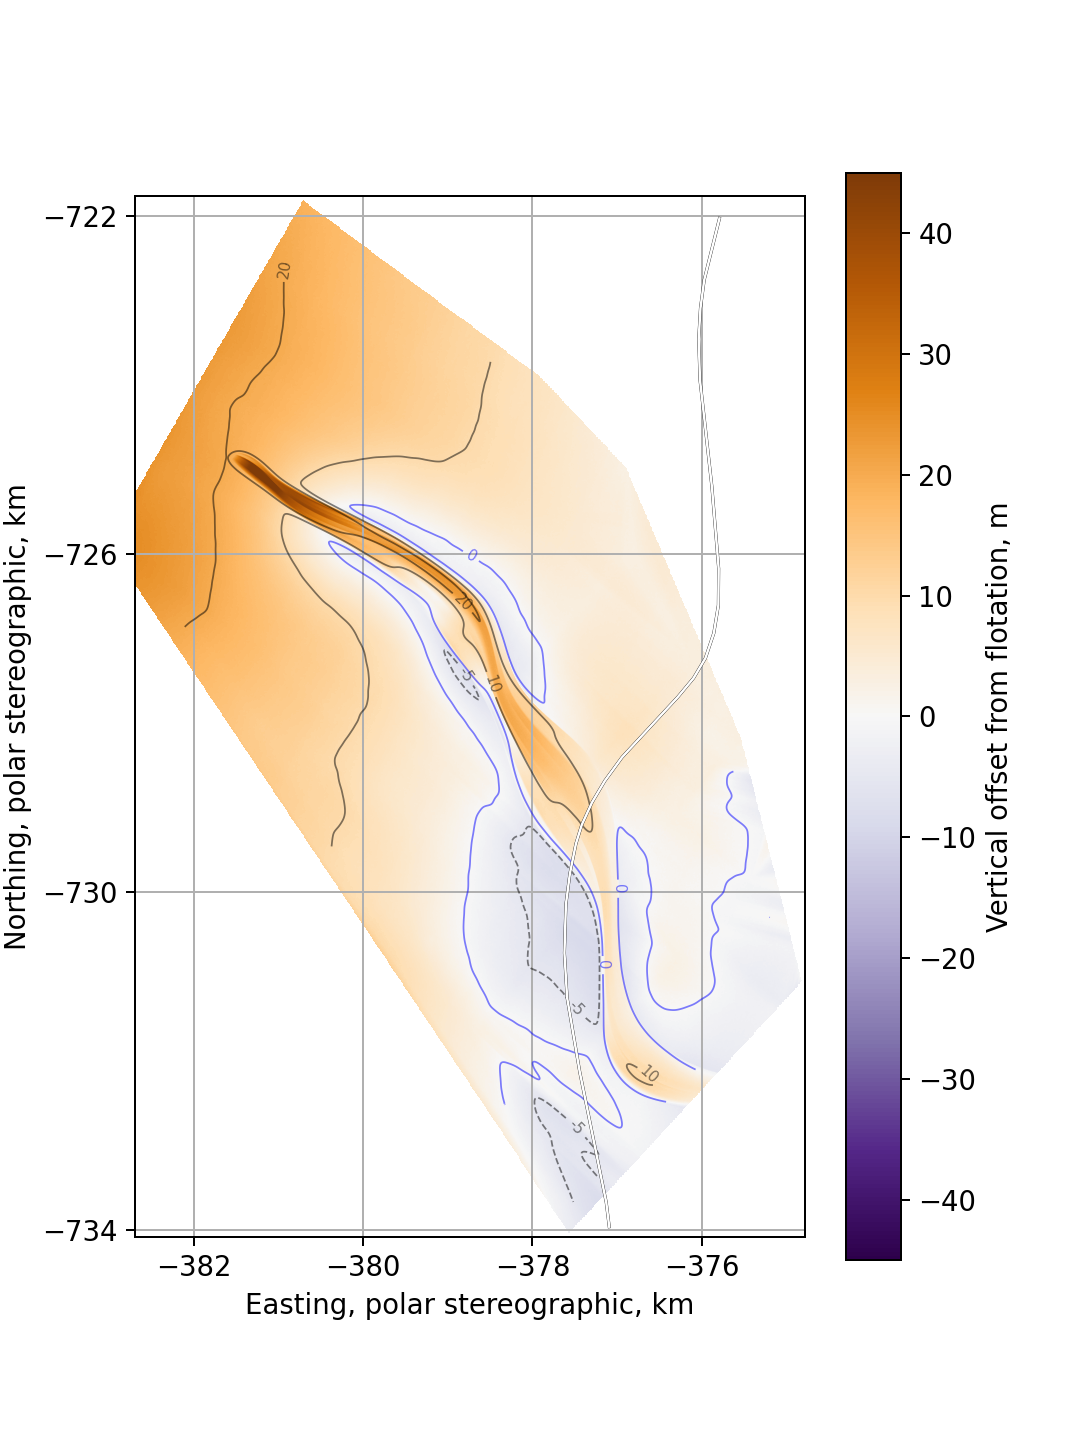
\includegraphics[width=0.9\textwidth]{chapters/2/where_float.png}
\caption[Hydrostatic Equilibrium]{Vertical offset from hydrostatic equilibrium. Blue line indicates the zero contour, where ice is estimated to be floating. Positive values indicate ice is held above floatation either by the ground, or by bridging stresses with surrounding ice. Negative values indicate ice is held below floatation by lateral stresses with surrounding ice.  White line is the grounding line from \cite{depoorter2013amii}. }
\label{fig:bridging}
\end{figure} 

\subsection{Surface elevation change } \label{sec:changeintopog}

\subsubsection{Change in surface topography} \label{sec:changeinsurf}


\begin{figure}[!ht]
\centering
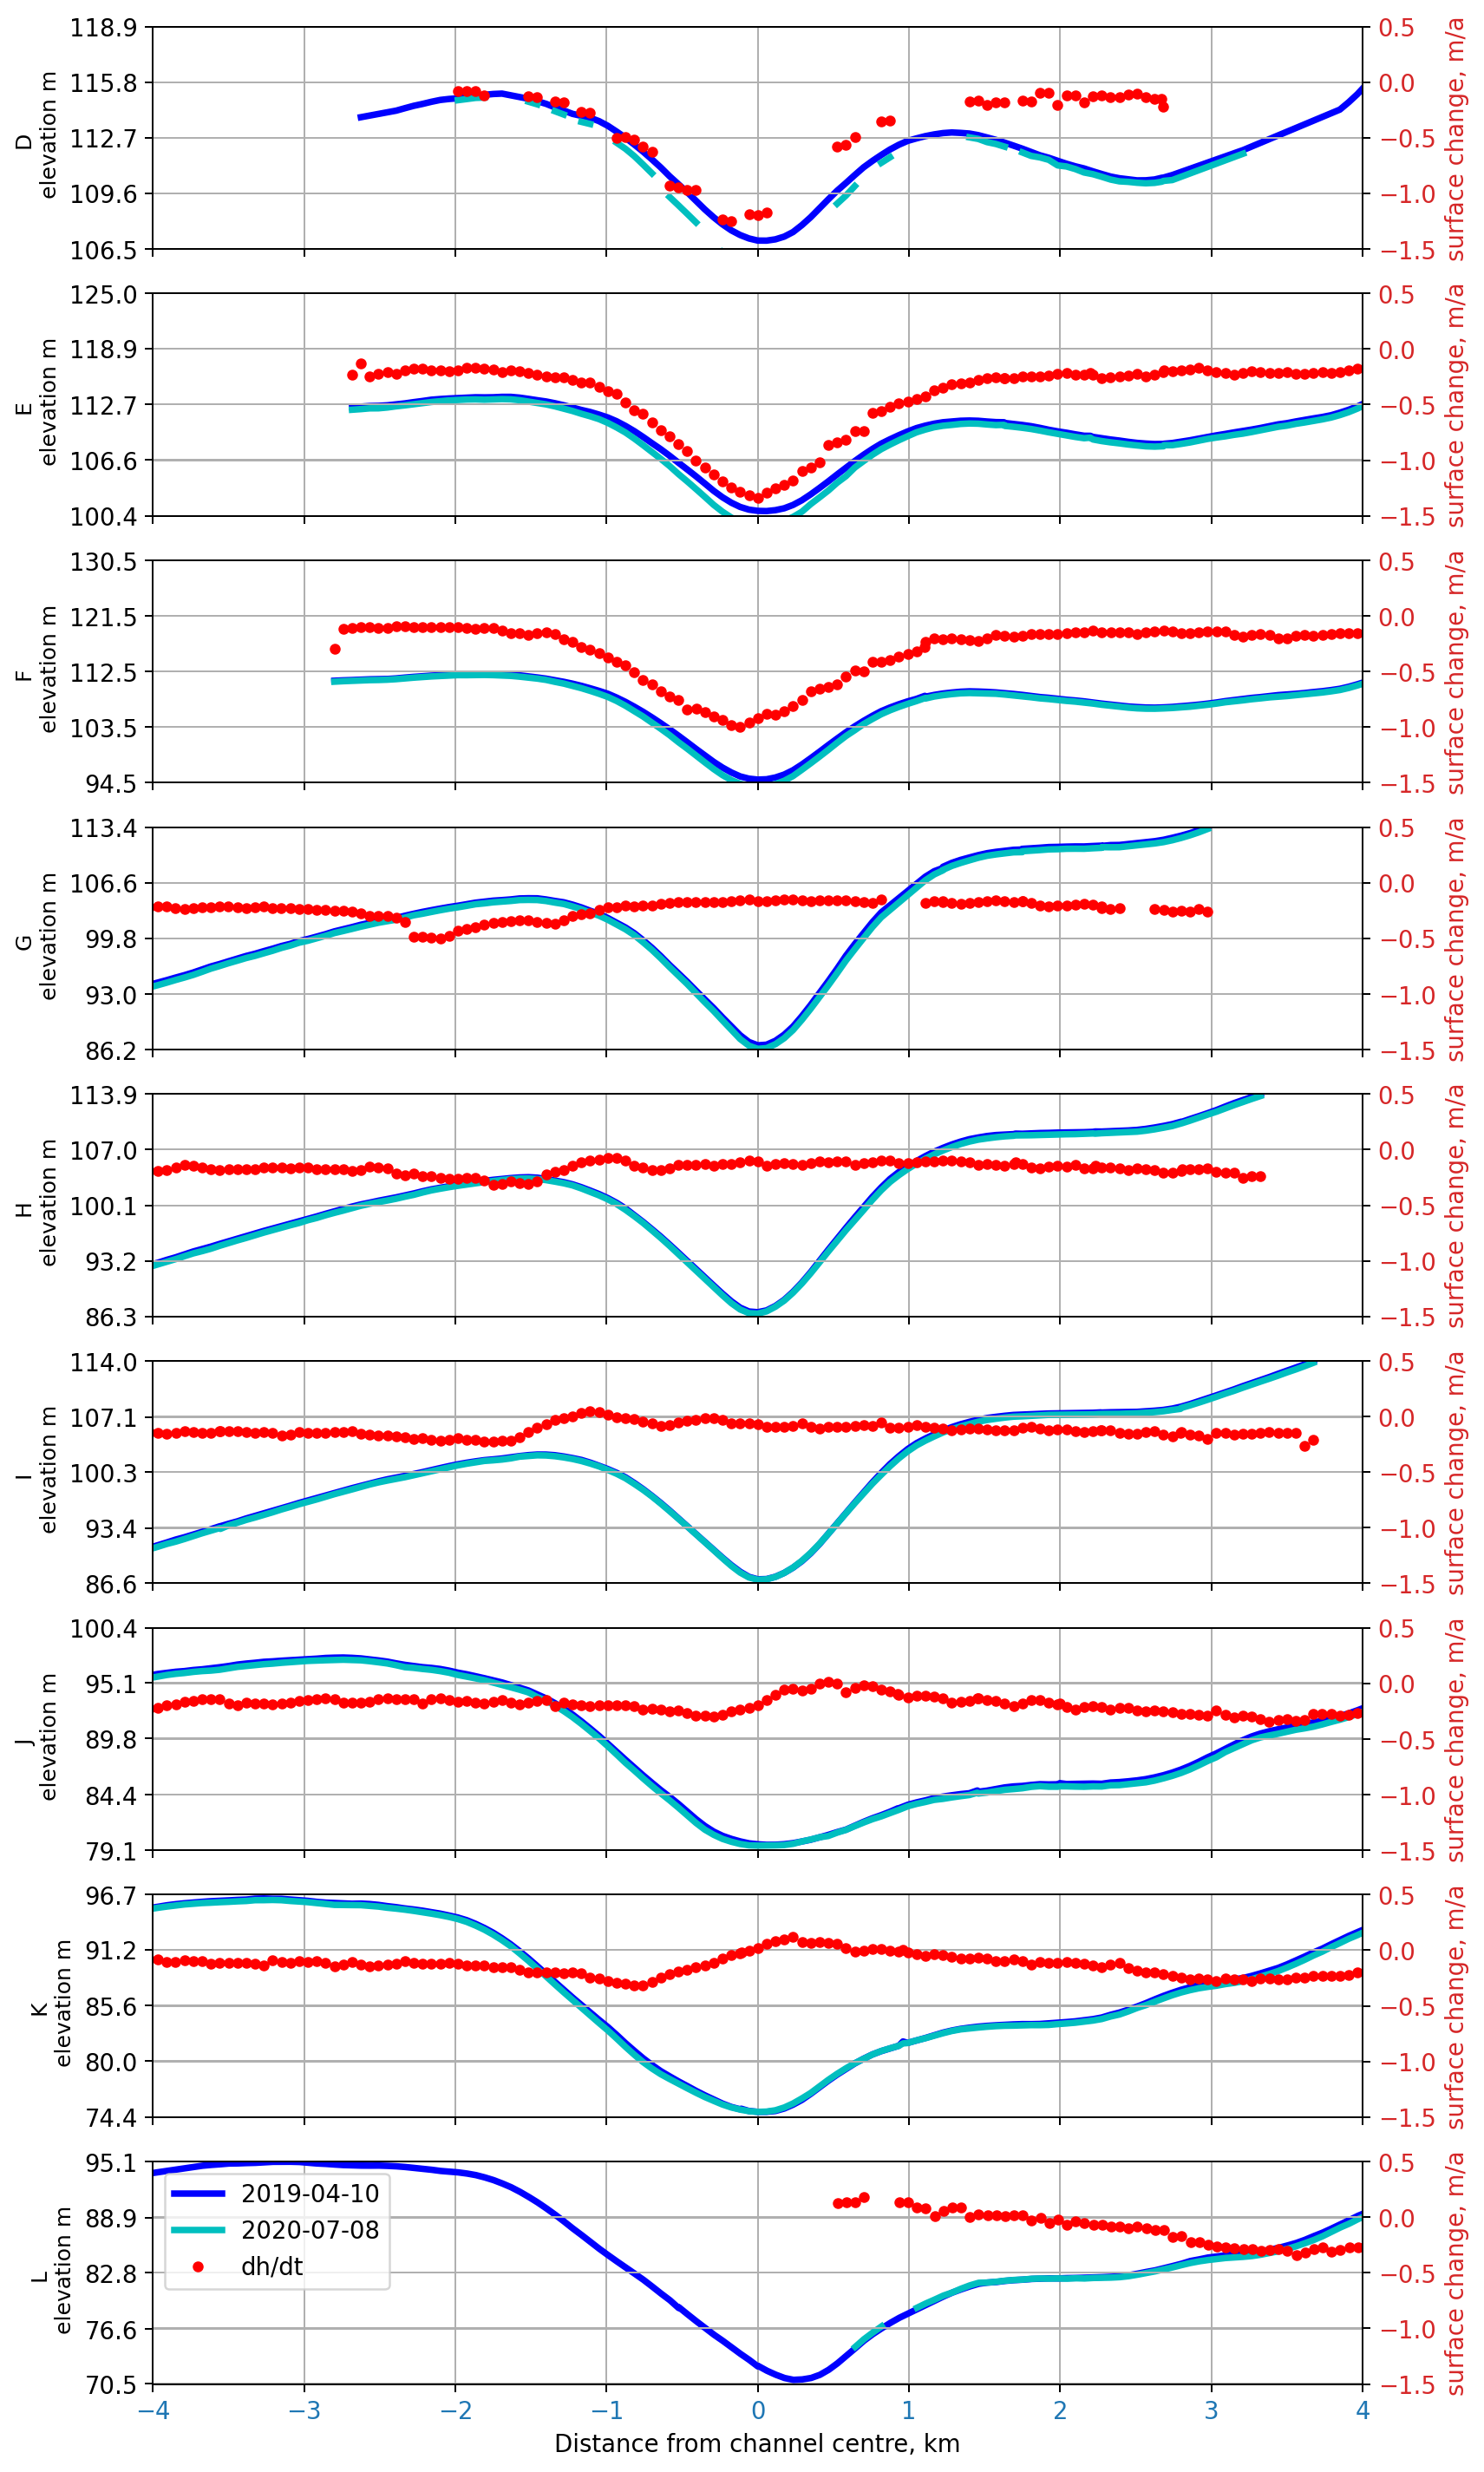
\includegraphics[width=0.7\textwidth]{chapters/2/icesat2_b.png}
\caption[ICESat--2 profiles]{ICESat--2 along track elevations and differences for nine tracks which cross the surface valley in 2019 and 2020. Locations of the lines are shown in Figure \ref{fig:geophysics_overview} and S4. Lines D to L are in order from upstream to downstream. Lines are shown looking downstream, positive distance from channel centre corresponds to true right.
 }
\label{fig:icesat2_b}
\end{figure}


Near the inception of the basal channel, a region of modern surface lowering is apparent when differencing REMA elevation strips from 2012-12-24 to 2016-11-09 (Figure  \ref{fig:4square_channel} D). The region of surface lowering is an oval approximately 1.4 km long in the along--channel direction and 1 km wide in the cross-channel direction. This region is centred around the onset of the surface valley (Figure \ref{fig:thickness_surfacecolour} B).  The first 300 m of the basal channel sits outside of the region of surface lowering  (Figure \ref{fig:thickness_surfacecolour}). Over the full difference image, shown as `Stable area' in Figures \ref{fig:REMA_histogram} and \ref{fig:REMA_broad}, the mean is 0.3 m/yr (surface raising) and the standard deviation is 0.2 m/yr, which we use as an estimation of uncertainty in the area. 

\begin{figure}[!ht]
\centering
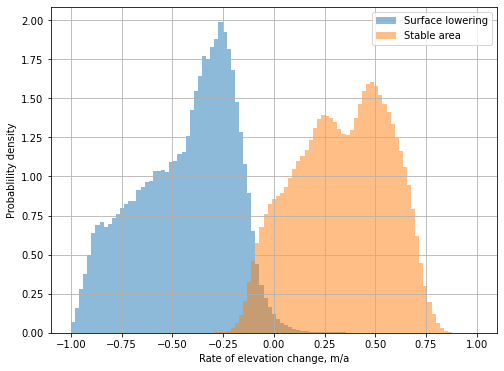
\includegraphics[width=0.9\textwidth]{chapters/2/REMA_histogram.png}
\caption[REMA difference distribution]{Histogram showing the distribution of the REMA rate of surface elevation change in two areas. The distribution of background elevation change distribution is shown in blue (`Stable area' outlined in Figure \ref{fig:REMA_broad}), and the region `Surface lowering' (outlined in Figure \ref{fig:REMA_broad}) is shown in peach.}
\label{fig:REMA_histogram}
\end{figure}

\newpage
The region of surface lowering is centred  approximately 1 km downstream from the onset of the basal channel (Figure \ref{fig:4square_channel} C, D). This region has a maximum of -1.0 $\pm$ 0.2 m/yr at its centre, and has a mean elevation change of -0.4 $\pm$ 0.2 m/yr (Figure \ref{fig:4square_channel} D).  Differences from ICESat--2 point elevations from 9 May 2019 to 5 August 2020 find the same pattern, showing surface lowering up to -1.25 $\pm$ 0.02 m/yr on three upstream lines that cross the circular region (Figure \ref{fig:icesat2_b} D, E, F). 
%ICESAT2 within 1/2 a km of the tip of the channel show surface down--wasting, slightly shifted grid north.
One kilometre downstream from this region, ICESat--2 point elevations show more complex changes in surface elevation (Figure \ref{fig:icesat2_b} G, H, I). While the background ice stream's surface is lowering at around -0.2 $\pm$ 0.02 m/yr, the surface valley's sides are lowering more quickly, with the true right side  lowering up to -0.4 $\pm$ 0.02 m/yr more than the background ice stream (Figure \ref{fig:icesat2_b} G, H, I).  This suggests that the channel is widening, but not deepening in this area.
Further downstream, the REMA strip difference shows up to 0.5 $\pm$ 0.2 m/yr increase in surface elevation along the true right side of the valley shown in Figure \ref{fig:4square_channel} D between (-379.5,-727) and (-377.5,-730). While this signal does not dominate uncertainty, the more accurate ICESat--2 differences confirm these elevation changes.  At the downstream end of this area (coincident with the basin B2 labeled in Figure \ref{fig:thickness_surfacecolour}), the later ICESat--2 differences from 2019--2020 (Figure \ref{fig:icesat2_b} J, K, L) show up to 0.1 $\pm$ 0.02 m/yr of increase in surface elevation on the true right of the valley and -0.3 $\pm$ 0.02 m/yr of lowering on the true left, suggesting that the valley is migrating to the true left. Background surface lowering on ICESat--2 lines J, K and L is between -0.1 $\pm$ 0.02 m/yr and -0.2 $\pm$ 0.02 m/yr (Figure \ref{fig:icesat2_b} J, K, L). This location is coincident with the location of ledge L2 (Figures S8, S9) discussed in Section \ref{sec:icebasetopog}. 
 

\subsubsection{Change in ice base topography} \label{sec:changeinbase}

While caution should be taken when interpreting accretion rate estimates from repeat ApRES observations, our observations indicate apparent accretion is occurring within the downstream portion of the basal channel (Figure \ref{fig:APRES_melt}). 
On the cross channel profile (see Figure \ref{fig:geophysics_overview} for the location), all but one of the ApRES survey sites outside the channel indicate basal melt. In the channel, all sites indicate apparent accretion. Apparent accretion peaks on the true right of the channel, coincident with a ledge (Figure \ref{fig:ledges1} L2) and surface raising detected by REMA strip differencing (Figure \ref{fig:4square_channel} D, Section \ref{sec:icebasetopog} and \ref{sec:changeinsurf}). ICESat--2 data also show surface raising on the channel right in a similar area (Figure \ref{fig:icesat2_b}). 
Vertical strain rates derived from ApRES observations map roughly to melt rates (Figure \ref{fig:APRES_melt}). Strain is most negative where accretion is strongest, and low melt rates map to sites with low strain. Two sites at the channel apex are an exception, where both accretion is strong and strain is close to zero.

%/DATA/Jupyter/APRES/plot_apres_melt.ipynb
\begin{figure}[!ht]
\centering
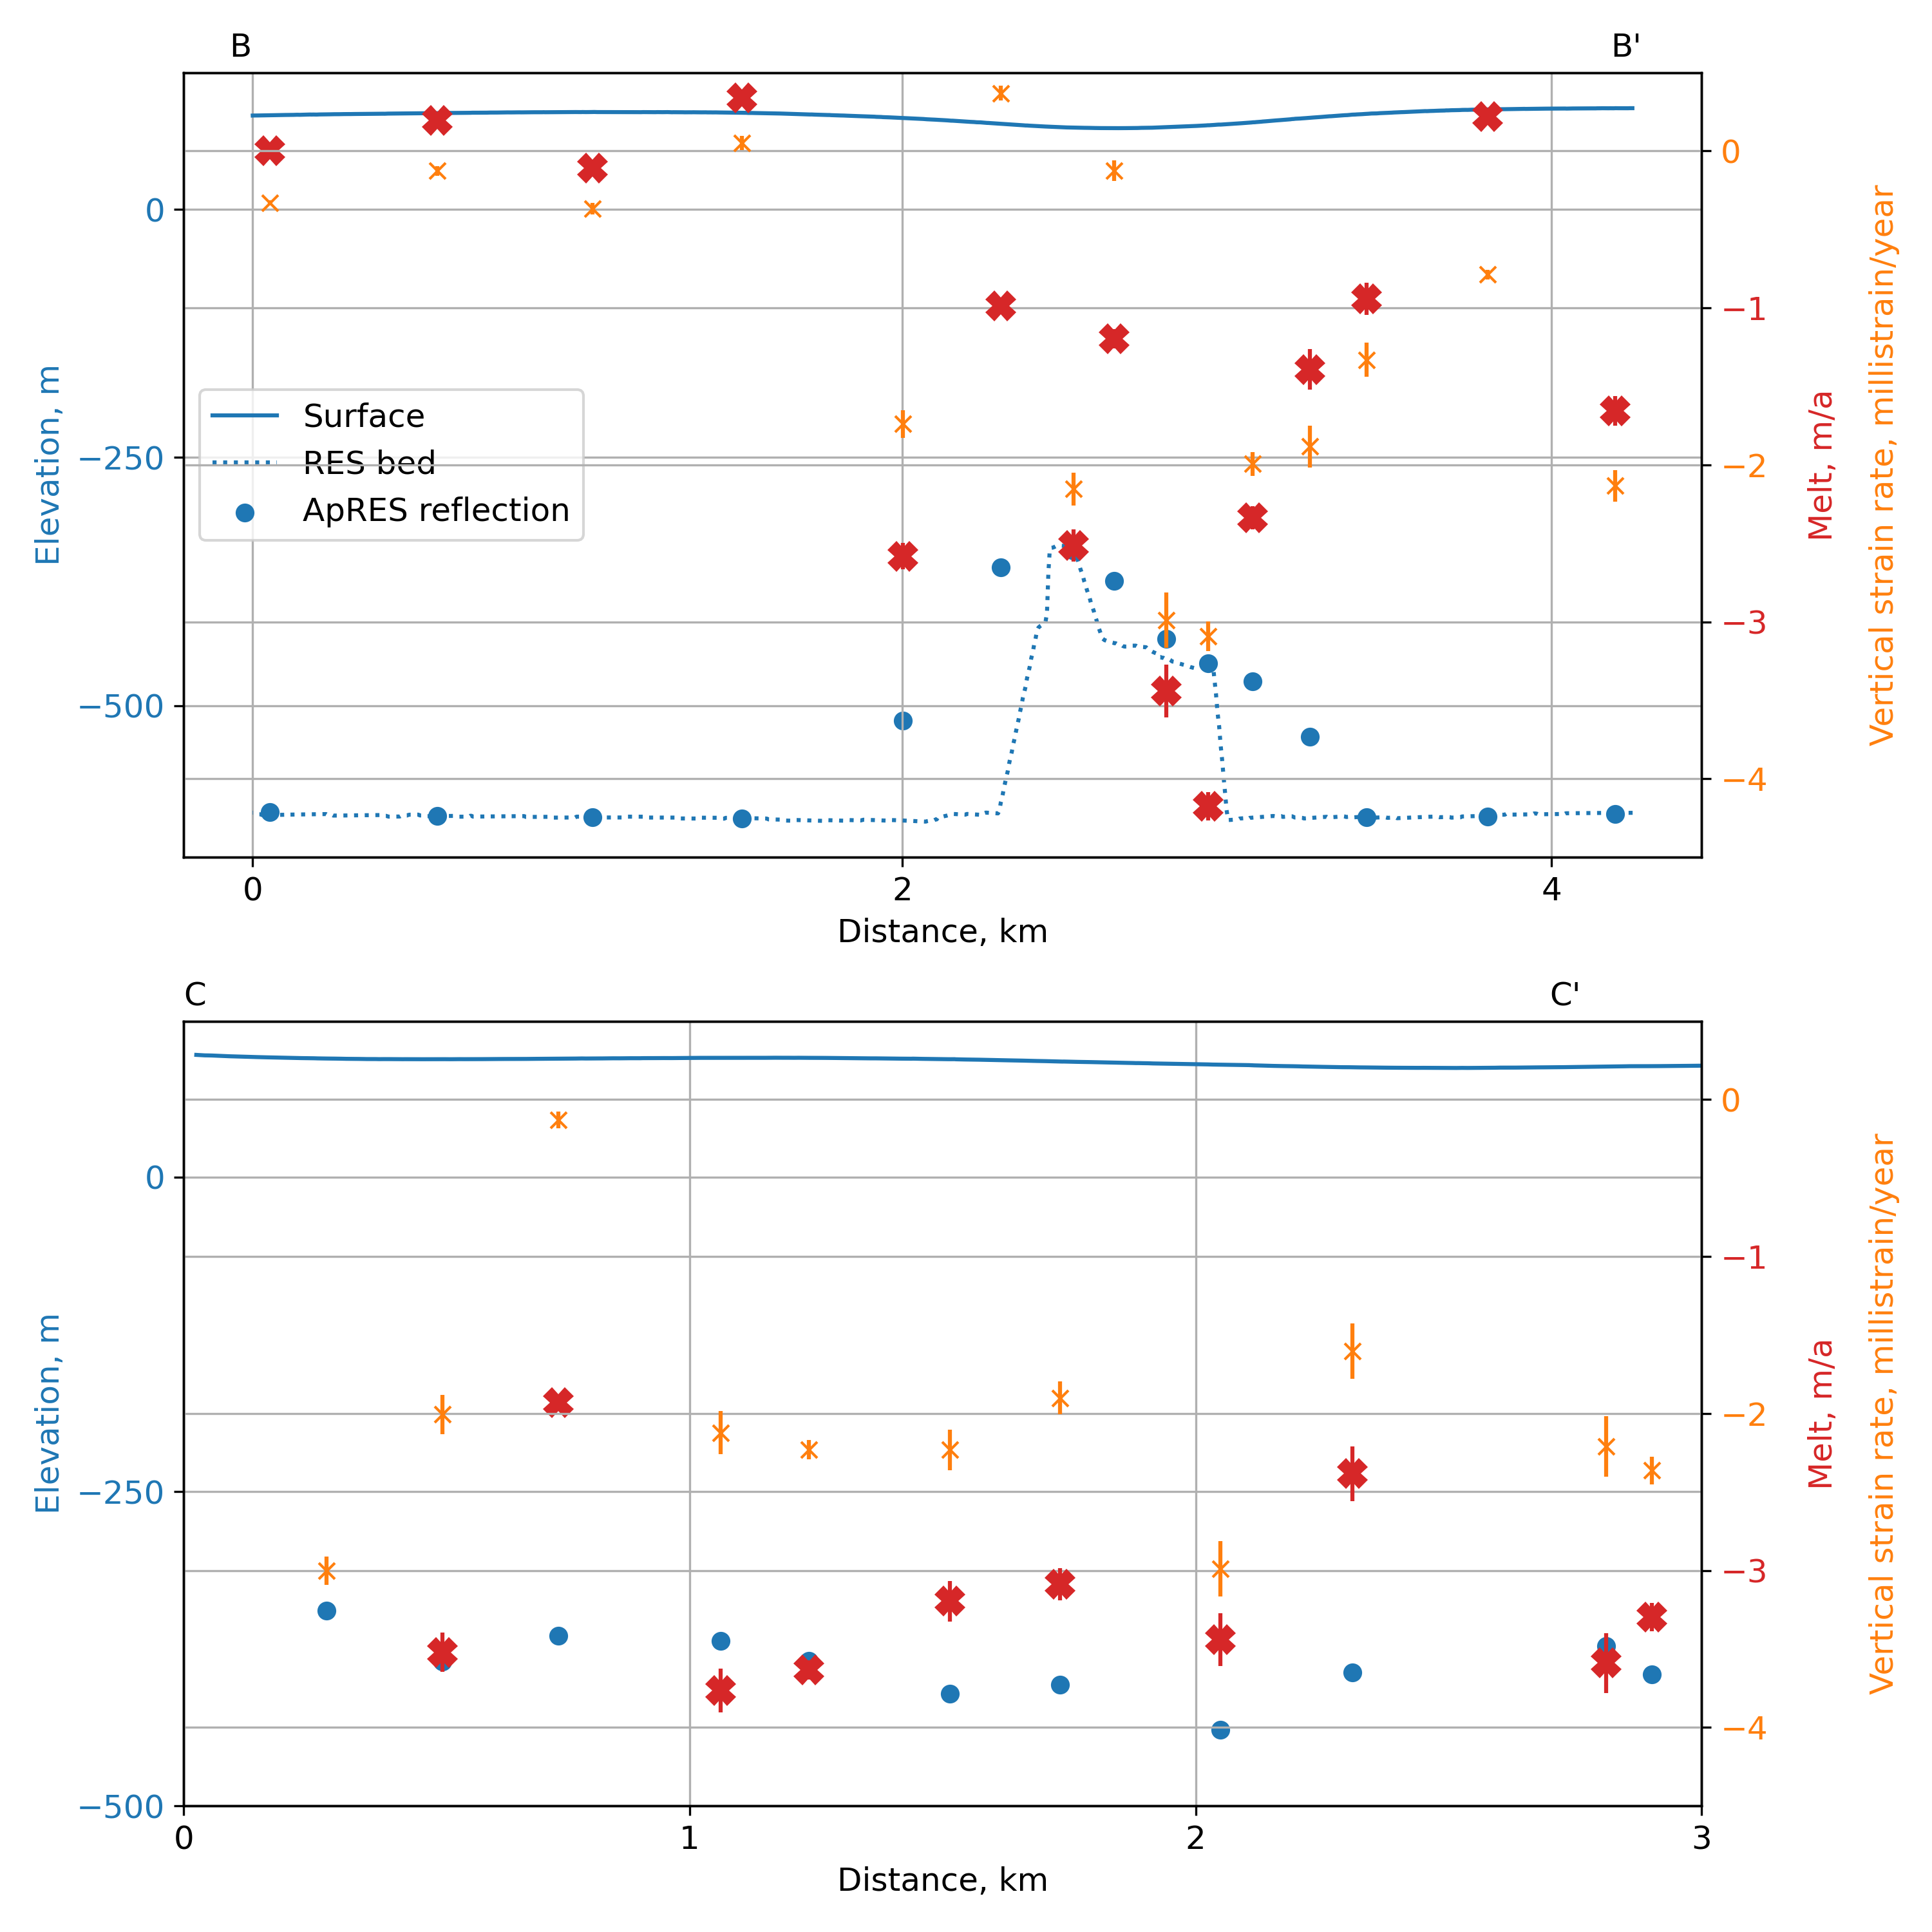
\includegraphics[width=1\textwidth]{chapters/2/APRES_melt.png}
\caption[ApRES results]{ApRES basal mass balance on two profiles the channel shown in (Figure \ref{fig:geophysics_overview}). `B' crosses the channel at right angles, `C' follows the surface valley low.  ApRES repeat surveys are from 07/12/2019 to 22/12/2020. Negative melt denotes accretion.   }
\label{fig:APRES_melt}
\end{figure}  

\newpage

\section{Discussion} \label{sec:discussion}


\label{sec:meltwater}

Our observations confirm that the surface valley described in Section \ref{sec:topography} is the expression of a basal channel as concluded by \cite{kim2016active} and \cite{alley2016impacts} (Figure \ref{fig:4square_channel}C). 
As the channel's location corresponds to predictions of concentrated subglacial flow (Figure \ref{fig:fieldwork_location}), it is most likely that the channel has been incised by a subglacially sourced meltwater plume. Under Kamb Ice Stream, subglacial meltwater has been modelled as concentrating in a single hydropotential low before flowing to the sea \citep{carter2012supply, le2013evidence}. When this freshwater meets the salty ocean it likely forms a buoyant plume which entrains warmer ocean water (as described by \cite{sergienko2013basal}), and incises the channel into the underside of the Ross Ice Shelf (Figure \ref{fig:4square_channel}). Plume driven melt incises the channel both higher into the ice and upstream following the subglacial drainage route. As the channel grows, the grounding line is shifted locally upstream, and salty bottom water flows upstream to replace fresh plume driven outflow in the top of the water column. The resulting shape and circulation is likely comparable to an esturine river mouth, whereby the sea and fresh water meet in a channel which forms a local deviation from the coast line. In addition to a classic estuary, a melt water plume at the inception of the channel directly couples fresh and salty layers by entraining the upstream flow of salty bottom water and expelling buoyant fresh water. 



\label{sec:surface_lowering}
We interpret the surface lowering (Figure \ref{fig:4square_channel} D) as caused by submarine melt and subsequent adjustment of the ice towards hydrostatic equilibrium. The region is approximately 2 $\mathrm{km}^2$ and the surface is lowering by up to approximately 1 m/yr. The along--channel orientation of the oval of surface lowering suggests melting is occuring over an elongated region of the channel, though the shape does not directly reflect the shape on the ice base. We attribute the general mismatch of surface and basal topography to bridging stresses in the ice.

\subsubsection{Bridging} \label{sec:bridging}

% Bridging
Ice bridging is indicated in Figure \ref{fig:4square_channel} C, as the basal shape is not mirrored directly at the surface. Surface changes shown in Figure \ref{fig:4square_channel} D suggest that melt induced changes to the basal shape are also not not mirrored directly at the surface, indicating bridging. The rigidity of ice distributes bridging stresses, whereby the weight of ice is partially supported laterally by the surrounding ice and ground. This smooths the surface response to basal changes at a length scale which masks small features. 
This is shown in Figure \ref{fig:bridging}, where in places the surface is above flotation on the channel and close to or below flotation to either side of the channel. Over larger regions ($\approx$ 1x1 km) the ice is adjusting to hydrostatic equilibrium, while over smaller length scales ($\approx$ 100x100 m) the ice is not at flotation. 
This is well supported by ice dynamics theory, which predicts that the length scale of surface expressions of the basal channel will be no smaller than the ice thickness  (shown in Figure \ref{fig:4square_channel}, $\approx$ 700 m at the field site) \cite [e.g.][] {gudmundsson2008limit}.
Significant bridging has been noted around other ice shelf channels, and used to explain discrepancies between basal and surface topography \cite [e.g.][] {dutrieux2013pine,chartrand2020basal,vaughan2012subglacial}. These explanations are supported by ice dynamics modelling by \cite{drews2015evolution}, who found that narrow channels show significant bridging, even at equilibrium. 


While further stress modelling would be required to understand in more detail where bridging stresses affect the surface expressions of the basal channel, our observations begin to explain how surface lowering is influenced by bridging. One conclusion is that more basal melt has occurred than that which is manifest in surface lowering. %indicating more melt occurs than is manifest on the surface.
In our study area, ice is furthest from hydrostatic equilibrium at the inception of the channel (Figure \ref{fig:bridging}), which is upstream from the surface valley (Figure \ref{fig:4square_channel}C). 
We expect basal melt to occur at the start of a positive basal gradient of ice, as theoretical models \cite [e.g.][] {jenkins2011convection} of sub--ice--shelf plumes assume these plumes are generated by buoyancy \citep{jenkins1991one}. These models predict that positive slopes at the ice base, like that at the head of the channel, will generate melting. 
However, the region of surface lowering does not overlap the inception of the channel but starts 300 m downstream from the initial channel ramp (Figure \ref{fig:thickness_surfacecolour}). 
We attribute this discrepancy to ice bridging and suggest that melt is occurring at the inception of the basal channel but is not expressed at the surface. Significant bridging is expected at the inception as it is just 200 m wide (shown in Figure \ref{fig:4square_channel}, similar to the channel modelled by \cite{drews2015evolution} and \cite{wearing2021ice}). As the channel inception grows wider over time, basal melt will likely be manifest at the surface as surface lowering. 
The 1000 m wide region of surface lowering (Figure \ref{fig:4square_channel}D) is much wider than the 200 to 400 m wide basal channel below, reflecting the fact that sharp changes to the base will be smoothed at the surface due to bridging  stresses which provide lateral support. While the area of the surface lowering may be larger than the area of basal melt, the volume of ice lowered on the surface is expected to be smaller than the basal volume melted due to lateral support in the ice.
ApRES surveying shows basal accretion at the edge of the large area of surface lowering (Figures \ref{fig:geophysics_overview}, \ref{fig:4square_channel}, \ref{fig:APRES_melt}). This likely shows that while basal melting and accretion are occurring within close proximity, the melt signal is overwhelmingly larger, and so is smoothed by bridging and masks the accretion signal at the surface.

\subsubsection{Quantifying basal melt} \label{sec:melt}

Despite the distorted representation of basal changes on the surface topography, we know that basal topography will be underrepresented at the surface but not over represented. It follows that we can estimate a minimum melt rate from REMA differences (Sec. \ref{sec:changeinsurf}). REMA and ICESAT--2 differences show surface downwasting of up to 1 and 1.25 m/yr respectively. In the same location \cite{kim2016active} used Landsat imagery to calculate 1.2 m/yr of surface lowering.
Integrating over the circular area of surface lowering shown in red in Figure \ref{fig:4square_channel} C, the ice volume lost is found to be 1,270,000 $\mathrm{m}^3$/yr. Calculating the submarine volume lost (assuming the lowering is from hydrostatic adjustment to equilibrium) and restricting the melted volume to the area of the channel, basal melt rates are estimated as approximately 20 m/yr. Due to uncertainties described below, this estimation is a lower bound on melt rates in the channel. In comparison, \cite{marsh2016high} and \cite{stanton2013channelized} used ApRES to measure melt rates of 22.2 $\pm$ 0.2 m/yr and 14.2 to 24.5 m/yr in channels on the ice shelves of the Whillans Ice Stream and Pine Island Glacier respectively. 
Figure \ref{fig:bridging} shows the region of surface lowering (delineated in Figure \ref{fig:thickness_surfacecolour} B) is not at hydrostatic equilibrium but is likely close to it, shown by the fact ice $<1$ km downstream, on either side of the channel (at -380,-726) is floating. 
The along-flow strain rate in the area is $< 2 \times 10 ^{-6}$/yr \citep{alley2018continent}, too small to produce such large surface changes. 
Our initial estimate likely underestimates melt. Firstly, our estimate neglects surface mass balance which is likely positive in the surface valley, due to the fact hollows tend to be filled in by wind driven snow \citep[e.g.][]{gow1965relationship}. Secondly, due to bridging stresses, the basal melt is understated at the surface \citep{drews2015evolution}. If ice is not at hydrostatic equilibrium at the channel ceiling, it is held away from hydrostatic equilibrium. Any melt in the channel will be expressed at the surface less than or equal to if it were at hydrostatic equilibrium, but not more. Thirdly, in calculating a 1D melt rate from a melt volume we assume melt spans the channel area. However, melt is likely restricted to a smaller area due to the Coriolis force which will cause the melt plume to trend to the true left wall (more detail in Section \ref{sec:side_melt}). A smaller melt area would correspond to a higher 1D melt rate for the same melt volume.  
Lastly, if the channel was filled with rock or till, the assumption that the channel roof was supported by bridging or floating may be wrong, and melt rate could be overestimated. However, due to the location of the channel in a drainage outlet, the large magnitude of surface lowering, and the fact that the region of lowering ice is close to flotation (Figure \ref{fig:bridging}), it is unlikely that the channel is not water filled. It follows that basal melt is most likely understated here.

REMA strips state a vertical accuracy of 4 m and 3.5 m for 2012 and 2016 strips respectively \citep{noh2015automated,howat2019reference}. Because the study area is relatively stable due to low surface velocity \citep{rignot2017measures}, both strips are expected to be more accurate than the large stated accuracy. This also applies to the uncertainty of the vertical offset from hydrostatic equilibrium (Section \ref{sec:floating}), which is calculated from the 2016 REMA strip.  While 4 m is large relative to the $\approx$ 5 m range we observe to calculate the rate of surface lowering, it is unlikely we have overstated surface lowering in the accuracy due to the following. Firstly, ICESat–2, with a mean accuracy of 1.12 cm shows a near identical region of lowering, with a similar magnitude (Figure S4). While the lowering shown in ICESat--2 spans a different time period, its similarities suggest that the process observed is ongoing. Secondly, the observed lowering is the opposite sign from the general trends and error in the data. The mean of the difference between REMA strips is positive (surface raising) over grounded ice outside the negative region of surface lowering (Figure \ref{fig:REMA_histogram}). Over the full difference image, the mean is 0.3 m/yr (surface raising) and the standard deviation is 0.2 m/yr, which we used to estimate uncertainty. In the region of lowering the mean surface change is -0.4 $\pm$ 0.2 m/yr. The mean lowering is therefore out of the range of the uncertainty. Thirdly, artifacts in the REMA difference show patterned bands which are clearly different to the observed surface lowering (Figure \ref{fig:REMA_broad}). The region of surface lowering is centred between bands, where background surface change is negative.

\begin{figure}[!ht]
\centering
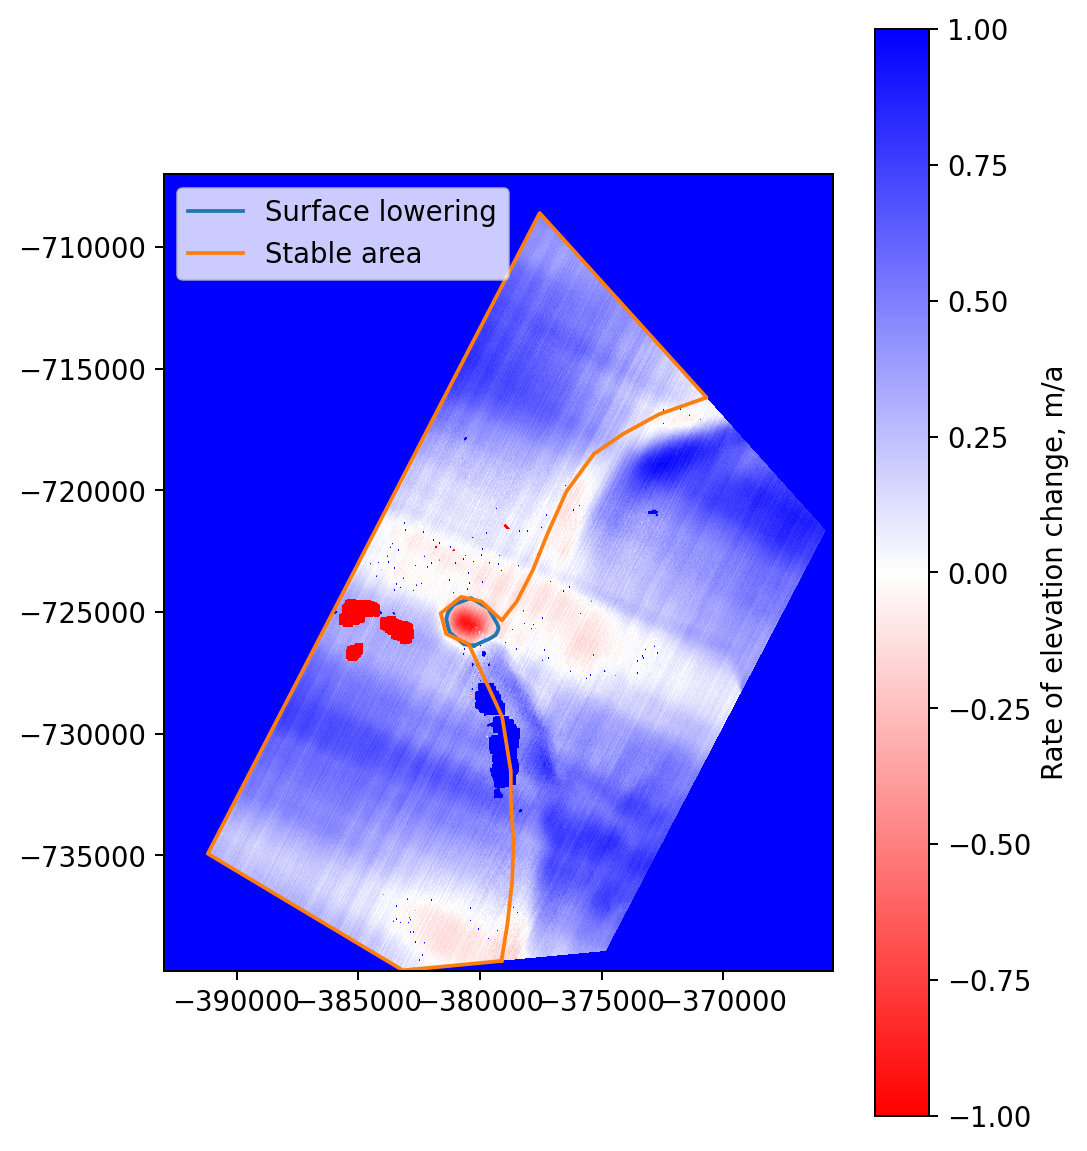
\includegraphics[width=0.9\textwidth]{chapters/2/REMA_broad.png}
\caption[Broad REMA difference]{Broader view of the difference between REMA elevations from 2012-12-24 to 2016-11-09 \citep{noh2015automated,howat2019reference} as in Figure \ref{fig:4square_channel}. Dark blue spots to the true--right of the channel, and red spots upstream of the area `Surface lowering' are artefacts.}
\label{fig:REMA_broad}
\end{figure}

\subsection{Mechanisms} \label{sec:shape}
\subsubsection{Stepped grounding line retreat} \label{sec:retreat}

With ice velocity less than 5 m/yr at the channel head \citep{rignot2017measures},  there is no clear mechanism to explain why the basal channel is a ($\>$10km) long feature. We suggest that the melt plume has migrated upstream, leading to the present linear channel shape.  
In Section \ref{sec:melt} we estimated modern melt rates to be over 20 m/yr vertically. At this rate, the basal channel would take less than 18 years to melt vertically through 350 m of ice to its current height.  The fact that melt is ongoing suggests that the channel exhibits large changes in melt rates, and/or channel melt migrates over time. Landsat imagery shows the surface valley migrates upstream (Figure \ref{fig:historic}), and REMA differences reveal modern melt is likely at the head of the channel (Figure \ref{fig:4square_channel} D).   Since 1985, the surface valley has grown upstream by 1.5 km towards the location of modern surface lowering (Figure \ref{fig:historic}, 2020).
Similarly, \cite{chartrand2020basal} observed a sub--ice--shelf basal channel migrating upstream towards a grounding line at $\approx$ 1 km/yr.
Surface elevation shows three distinct basins in the surface valley (B1, B2, B3, Figure \ref{fig:thickness_surfacecolour}). These basins are clear in the oldest satellite imagery of the valley (Figure \ref{fig:historic}, 1985). We interpret the surface basins to be historic plume locations and suggest that the modern grounding line and meltwater plume location is situated just upstream of the surface lowering shown in Figure \ref{fig:4square_channel} D. 

We suggest that the basin features are formed by varying melt from either or a combination of the two processes proposed by \cite{horgan2017poststagnation} to describe disjointed channel features in the area. Either melt rates vary in time or the region's grounding line has undergone stepwise retreat.
Large changes in melt rates could result from changes in flux in the subglacially sourced meltwater plume. Changes in plume flux could be caused by episodic subglacial drainage events upstream, originating from the flooding of upstream active subglacial lakes as described by \cite{kim2016active}, or in changes in flux caused by the rapid rerouting of the subglacial network as described by \cite{carter2012supply}. Maximums in subglacial outflow would cause a strengthening of the subglacial plume, allowing melt to occur higher in the water column. Wider parts of the channel likely form between melt peaks, when a weaker plume melts the channel walls.
%Maximums in subglacial outflow would cause temporal peaks in melt, creating the wider parts of the channel associated with the surface basins we describe. 
While changes in ocean conditions could similarly cause fluctuations in melt rates due to the dependance of melt on the amount of heat and salt entrained from the ocean \citep{jenkins1991one}, conditions in the ice shelf cavity interior are expected to be stable \citep{stevens2020ocean}. 
Alternatively, the region's grounding line could be retreating episodically. At each step, the steep plume would melt a hollow, manifest in a basin shape on the ice surface.
 Stepwise retreat can occur when the grounding line jumps between stable positions usually determined by local bed topography \citep{haseloff2018effect}, and is commonly observed \cite [e.g.][] {jakobsson2012ice}.  
 

The channel bends and corresponding changes in channel width could be interpreted as channel meandering, similar to that of a supraglacial river \cite [e.g.][] {ferguson1973sinuosity}. 
At wider parts of the channel, the ice shelf has less buoyancy and so would locally sink, and would likely manifest as the basins at the surface seen in Figure \ref{fig:4square_channel}. However, we do not think meandering is a robust explanation for the channel shape, as it is unlikely the plume melts down the length of the channel in a manner similar to a supraglacial river. 
Firstly, the channel walls widen both left and right at bends rather than just on the outside of a bend like a supraglacial river \citep{ferguson1973sinuosity}.
Secondly, plume theory predicts that downstream from the initial positive gradient of the channel, the plume will not melt basal ice. Past this point, the plume will either cause accretion, as observed in ApRES observations (Figure \ref{fig:APRES_melt}), or detach from the ice.  It is possible that downstream from the positive gradient in ice basal slope at the head of the channel, subsequent plumes are generated from ice slopes on the walls or from downstream positive gradients in the channel depicted in Figure \ref{fig:thickness_surfacecolour}. 

The moniliform shape of the surface valley is similar to the shape of a feature observed by \cite{berger2017detecting} (Figure 7) at the Roi Baudouin Ice Shelf, Antarctica. Radar imagery shows this is the surface expression of englacial lakes found 30 m below the surface. While the basins we see are not formed by englacial lakes, it is interesting to note that this shape of connected basins in ice shelf topography appears to be stable. 

\cite{horgan2017poststagnation} propose that the grounding line retreated to its current location after the stagnation of the Kamb Ice Stream. The basal channel likely formed after this shift in the grounding line. 
Due to its location in a hydropotential low \citep{le2009subglacial}, the basal channel may have existed under grounded ice before Kamb Ice Stream's stagnation. As the grounding line retreated to its current location, feedbacks with the ocean likely allowed it to grow to its current size. Once ice advection stopped, even if  melt rates were low, the plume would be concentrated in one location allowing it to incise a deep channel. With no upstream migration of the channel, the observed 10 km long surveyed section of the basal channel would take approximately 2000 years to form with present ice velocity ($\approx 5$ m/yr). The channel continues downstream from the study area shown in Figure \ref{fig:4square_channel} C, though surface imagery shown in Figure \ref{fig:moa_solo} suggests that the basal channel is less pronounced.
It is possible that a strengthening of the meltwater plume is related to a proposed reorganisation of the subglacial drainage \cite [e.g.][] {anandakrishnan1997stagnation}, which may be associated with the ice stream shut down around $150$ years ago. For example, if the subglacial hydrology of the Kamb ice stream became more channelised as proposed by \cite{lelandais2018modelled}, subglacial flux at this location would increase. More buoyant subglacial water would be discharged at the grounding line, which would strengthen the sub--ice--shelf plume.  
% However, \cite{horgan2017poststagnation} highlight relict channels at a previous grounding line downstream, suggesting that channels formed at the grounding line of the Kamb Ice Stream before it stagnated.


\subsubsection{Steep initial channel slope} \label{sec:steep}

The initial gradient of the ice base at the inception of the channel in the downstream direction is constrained between $45^{\circ}-90^{\circ}$ by radar echo sounding observations (Figure \ref{fig:thickness_surfacecolour}).  This implies that the plume was flowing upwards at a steep or vertical angle when it incised the head of the channel. We suggest that the channel grows through a positive feedback between basal steepness and melt as described by \cite{sergienko2013basal} and \cite{gladish2012ice}. Through this feedback, steep basal slopes cause the plume flow to accelerate, which causes more melt, making preexisting slopes even steeper. 
In other observed ice shelf channels \cite [e.g.][] {drews2017actively, jeofry2018hard}, the height of incision is moderated by ice advection which restricts the amount of time any region on the ice shelf base experiences melt. 
In our study location, ice velocity is less than 5 m/yr at the channel head \citep{rignot2017measures}. Any notch melted into the ice shelf is not advected downstream but grows deeper over time, resulting in a steep gradient at the channel inception. Unless the plume changes, the feedback between slope and melting can continue until the channel is vertical at its inception \citep{sergienko2013basal,gladish2012ice}. The roof of the basal channel follows roughly the same elevation of around -380 m (Figure \ref{fig:thickness_surfacecolour}). This may represent a natural limit to which the freshwater plume will rise given the ocean density structure. A natural bound on the thickness of the channel should correspond to the height at which the plume reaches the density of the surrounding ice shelf cavity. Here, melt--water plumes are expected to stop rising and detach from the ice, flowing horizontally into the sea \citep{jenkins2011convection, hewitt2020subglacial}.


\subsubsection{Channel migration} \label{sec:side_melt}

Both REMA (Figure \ref{fig:4square_channel} D) and ICESat--2 data (Figure \ref{fig:icesat2_b} G--L),  shows less negative surface lowering (relative raising) just to the true right of the surface expression apex, and more negative surface lowering (relative lowering) on the true left of the surface apex. 
The relative rising surface is likely related to the accretion shown at the base of the channel by our ApRES observations (Figure~\ref{fig:APRES_melt}), which indicate more accretion is occurring on the true right of the channel. This  is coincident with a ledge (L2, Figures S8) described in Section \ref{sec:icebasetopog} . 
The Coriolis force likely causes the melt plume to follow the true left wall. This may be accompanied by accretion on the true right side, resulting in the leftward migration of the channel.   While it is not commonly observed that channels migrate to the left, \cite{gourmelen2017channelized} and \cite{alley2016impacts} found steeper walls on the true left of channel profiles and attributed the asymmetry to enhanced melt due to the Coriolis force. Similarly, \cite{chartrand2020basal} observed the leftward migration of a channel at $\approx$ 80 m/yr.
Our basal channel profiles show asymmetry in that the channel has large ledges on the right hand side for roughly half of the distance down the channel (Figure \ref{fig:ledges1}). Ledges (terraces) were also found on an ice shelf channel by \cite{dutrieux2014basal}.  \cite{drews2020atmospheric} also observed a pattern of surface lowering and raising across an ice shelf channel, and interpreted this pattern to be caused by wind eroding snow from windward slopes and depositing it on the leeward side of slopes. 
% While the pattern we observe may be caused by a combination of ablation and accumulation of surface snow, we do not have the observations needed to test this hypothesis. 

Relative to the ApRES data, REMA and ICESat--2 observations of a rising surface span a different time period and location respectively. However, both REMA and ICESat--2 show a consistent trend of a rising surface on the channel right (Figure \ref{fig:4square_channel} D, and Figure \ref{fig:icesat2_b} G--L). ApRES accretion and the surface rising shown in REMA/ICESat--2 occur downstream from the region of surface lowering we attribute to melt (Figure \ref{fig:4square_channel}D). This agrees with plume theory, which predicts that as a plume loses energy it causes accretion, downstream from where melt is occurring \cite{jenkins1991one}. Estimating the location of accretion with the 1D model of \cite{jenkins2011convection} is not done here as the oceanographic variables (e.g. ambient stratification in the ocean cavity) are unknown to us, and result in large changes in the length scale over which accretion occurs. 

\section{Conclusion} \label{sec:conclusion}
We have presented a series of observations describing a sub--ice--shelf channel at the grounding line of Kamb Ice Stream, combining remote sensing and field-based geophysical surveying. 
These observations reveal a channel that is actively melting at its upstream inception and has been growing upstream past the grounding line since at least 1989.
The inferred melt is likely driven by a buoyant plume, initiated by freshwater from Kamb Ice Stream's largest subglacial drainage outlet.
The channel is asymmetric and tortuous, unlike most observed sub--ice--shelf channels which tend to be linear and symmetric. While most sub--ice--shelf channels are formed as downstream streak lines in advecting ice, the channel we present is situated in stagnant ice, and appears to have developed its elongated shape due to a shift in the melt location. Over--snow radar surveying shows that the channel widens 50\%--100\% at each bend. The bends correspond to a moniliform series of basins on the surface which we relate to past locations of concentrated melt. 
We interpret the bends and basins as evidence that the upstream migration of the melt location at the head of the channel is irregular, stepping upstream over time. 
This irregularity likely stems from episodic subglacial drainage and/or instabilities in grounding line locations associated with bed topography. Radar surveying also reveals that the channel inception extends upstream of its surface expression. 
Ice above this narrow (250 m wide) part of the channel is not floating but is supported by bridging to the flanks of the channel. 
Modern melt is manifest as surface lowering. By quantifying this surface lowering, we estimate melt to be at least 20 m/yr. In agreement with channel theory, melt occurs near the upstream inception of the channel, and ice is accreted onto the channel roof downstream. This accretion is verified with ApRES observations and appears to be contributing to the growth of a ledge in the channel. The differences between the surface expression and basal features of this channel are noteworthy for studies of sub--ice--shelf channels using surface observations alone. To predict the stability of ice shelves, it may be important to model sub--ice--shelf channels. Our observations can be used as a case study to further constrain theories of channel formation and growth. As the channel shape is not distorted by advection, it serves as a natural experiment for understanding plume driven melt.
The results presented show that melt can form an ice shelf channel in the absence of advection through the inland migration of a focused melt source. Migration has continued upstream from the local grounding line, similar to an esturine river mouth. The focused melt source appears to continue to deepen and steepen the channel at its inception.
Future research on this channel could build on the work of this paper by better constraining melt rates and ocean plume properties, which in turn could be used to better understand subglacial outlet flow. This was the objective of a direct access drilling campaign carried out in the austral summer of 2021/2022.


%%%%%%%%%%%%%%%%%%%%%%%%%%%%%%%%%%%%%%%%%%%%%%%

% \section{Open Research}

% Low frequency radar data  used in Section \ref{sec:radar} are available at OneDrive via (\url{https://tinyurl.com/mss2uhrd}) with password whiteford2021. 
 
% % https://tinyurl.com/mss2uhrd
% %  https://vuw-my.sharepoint.com/:u:/g/personal/whitefar_staff_vuw_ac_nz/EUARLwFGT9lHhs3VDqDRYJ8Bg7Mw6L4fAuJge27vb0e5Lg?e=5fyBI5

% Accompanying code and notebooks used for radar processing and analysis are available at OneDrive via (\url{https://tinyurl.com/4bdb88fw}) with password whiteford2021.
% % https://tinyurl.com/4bdb88fw
% % https://vuw-my.sharepoint.com/:f:/g/personal/whitefar_staff_vuw_ac_nz/EloTtsJH8s1BlnmGe9WDUiMBI8EUVaJ48nq8fJDD7UPBYQ?e=Q9v4Xn 

% Repeat ApRES data used in Section \ref{sec:apres} are available at OneDrive via (\url{https://tinyurl.com/5d6wrak3}  with password whiteford2021.
% % https://tinyurl.com/5d6wrak3
% % https://vuw-my.sharepoint.com/:f:/g/personal/whitefar_staff_vuw_ac_nz/EpbPgKnipOtMv70lUkpQjpEBbzY3kmAf6m-ynq58KcIDrg?e=zWqPq3

% The above repositories are only intended for use to support the peer review process.
% These datasets will be made open access on Zenodo and Github with accompanying DOIs after the review. 


% RADAR
% picked_bed
%%%%%%%%%%%%%%%%%%%%%%%%%%%%%%%%%%%%%%%%%%%%%%%




